\documentclass[12 pt ,a4 paper, openright, oneside]{article}
\setlength{\marginparwidth}{2cm}
% Pacchetti %
\usepackage[utf8]{inputenc}
\usepackage{csquotes}
\usepackage{hyperref}
\usepackage{hyphenat}
\usepackage[hypcap=true]{caption}
\usepackage{setspace}
\usepackage[hang,flushmargin,bottom]{footmisc}
\usepackage{todonotes} % Note Todo
\usepackage{soul} % strikethrough 
\usepackage{caption}
\usepackage{amssymb,amsmath}
\usepackage[official]{eurosym}
\usepackage{frontespizio}
\usepackage{subfigure}
\usepackage{float}
\usepackage{listings}
\usepackage{xcolor}
\usepackage{amsmath}
\usepackage{tabularx}
\usepackage{amsfonts} 
\usepackage[T2A,T1]{fontenc}
\usepackage[russian, english]{babel}

% Tabelle %
\usepackage[normalem]{ulem}
\useunder{\uline}{\ul}{}
\usepackage{array,ragged2e}
\usepackage{colortbl}
\newcolumntype{P}[1]{>{\RaggedRight\arraybackslash}p{#1}}

% Immagini %
\usepackage{graphicx, wrapfig, float, rotating, subfigure}

% \graphicspath{{images/}}


% Language setting
% Replace `english' with e.g. `spanish' to change the document language
\usepackage[english]{babel}
% Set page size and margins
% Replace `letterpaper' with`a4paper' for UK/EU standard size
\usepackage[letterpaper,top=2cm,bottom=2cm,left=3cm,right=3cm,marginparwidth=1.75cm]{geometry}

% Useful packages
\usepackage{amsmath}
\usepackage{graphicx}
\usepackage{float}
\usepackage{hyperref}
\usepackage{amsfonts}
\usepackage{algorithm2e}
\begin{document}
\include{frontespizio.tex}
\tableofcontents
\include{intro.tex}
\section{Information Visualization}
La visualizzazione delle informazioni è un modo per comunicare significativamente i dati e aiutare le persone a 
dare un senso a grandi quantità di informazioni.
Le visualizzazioni come artefatti cognitivi che consentono il trattamento parallelo delle informazioni.
Tre scopi principali della visulizzazione:
\begin{itemize}
    \item \textbf{Explanatory}: Le visualizzazioni esplicative sono strumenti per presentare informazioni, comunicare dati e messaggi, spiegare qualcosa a qualcun altro.
    \item \textbf{Exploratory}: Le visualizzazioni esplorative sono strumenti per i lettori per analizzare ciò che viene loro presentato. Molto spesso, l'esito dell'analisi esplorativa non è solo la risposta alle domande originali, ma la generazione di nuove domande.
    \item \textbf{Confirmatory}: Nell'analisi confermativa, le visualizzazioni sono destinate a testare ipotesi.
\end{itemize}

Bisogna decidere cosa visualizzare 
\begin{figure}[H]
    \centering
    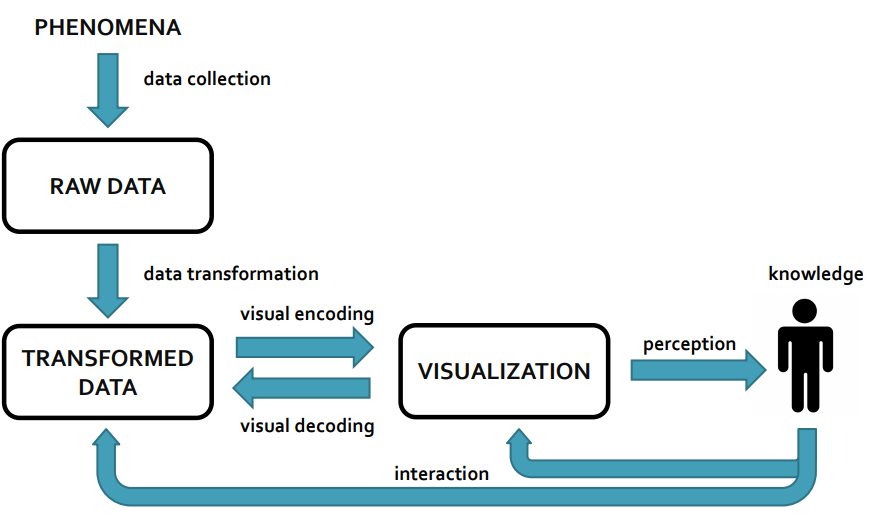
\includegraphics[width=0.5\textwidth]{images/visPipe2.png} % Sostituisci 'nome_immagine' con il nome del tuo file immagine
    \caption{Visualization pipeline}
    \label{fig:immagine}
\end{figure}
\subsection{Data}
Informazioni fattuali come misurazioni o statistiche, utilizzate come base per il ragionamento, la discussione o il calcolo.
I dati sono collezioni di \textit{items} e \textit{attributes} degli items.
Gli \textit{Items} sono gli oggetti/entità che vogliamo viusalizzare.
Gli \textit{Attributi} sono le proèrietà degli oggetti/entità.

Una \textit{Tabella} è una griaglia di colonne e righr, dove le righe  rapresentanto gli item e le colonne gli attributi.
Un \textit{network} è una collezione di nodi che rappresentano gli item, connessi tramite dei link; entrambi nodi e link possono avere attributi.

\subsection{Tipi di attributi}
\begin{itemize}
    \item \textit{Quantitativi}: sono gli attributi dove i valori rappresentano quantità misurate, 
        questi valori possono essere ordinati, ma può essere calcolata anche la distanza tra i valori.
    \item  \textit{Categorici}: sono gli attributi dove i valori descrivino le categorie,
        possono essere di tre tipi, \textbf{Nominali} se non hanno un ordine particolare, \textbf{Ordinali} se possono essere ordinati,
        \textbf{Binary} se hanno solo due stati.
\end{itemize}
\subsection{Semantica degli attributi}
\begin{itemize}
    \item \textbf{Spaziali e temporali}: Esempio la location, latitudine e longitudine o la data di assunzione come attributo temporale.
    \item \textbf{Sequnziali, ciclici divergenti}: Esempio: i mesi dell'anno sono ciclici, la temperatura è un attributo divergente.
    \item \textbf{Gerarchici}: Tipi di prodotto con sottocategorie, un esempio sono i vestiti.
\end{itemize}
Si deve selezionare la visualizzazione appropriata a seconda del tipo e dalla semantica dell'attributo.
Esempio:
\begin{figure}[H]
    \centering
    \begin{minipage}{0.45\textwidth}
        \centering
        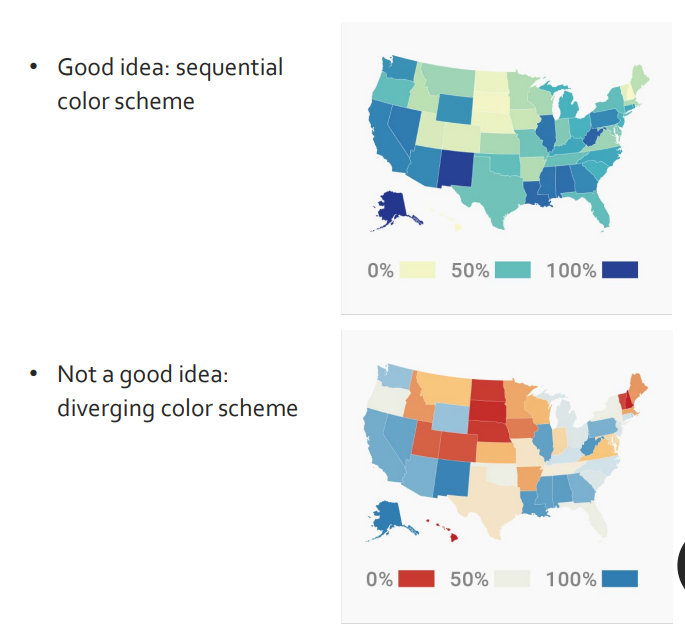
\includegraphics[width=\linewidth]{images/Attrubtevis.png} 
        \caption{Differenza di Visualizzazione}
        \label{fig:immagine1}
    \end{minipage}\hfill
    \begin{minipage}{0.45\textwidth}
        \centering
        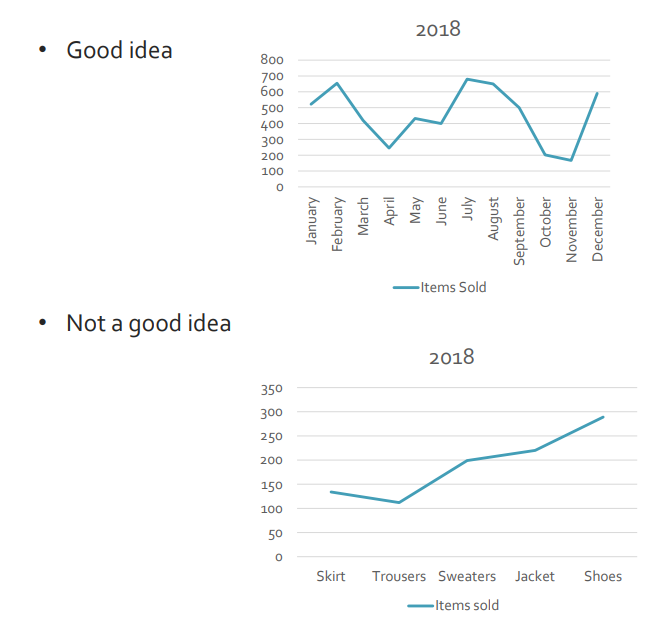
\includegraphics[width=\linewidth]{images/Attributevis2.png} % Sostituisci 'immagine2' con il nome del tuo file immagine
        \caption{Differenza di Visualizzazione}
        \label{fig:immagine2}
    \end{minipage}
\end{figure}
\subsection{Grafici Fondamentali (Bivariate data)} %--------------------------------------------------------------------------


\subsubsection{Bar Charts}
Visualizza come una quantità misurata si distribuisce tra categorie. Ogni barra rappresenta una categoria e la lunghezza della barra è una quantità misurata in quella categoria. Dati bivariati: nominale/ordinale e quantitativo.
 Non confondere con gli istogrammi
\begin{figure}[H]
    \centering
    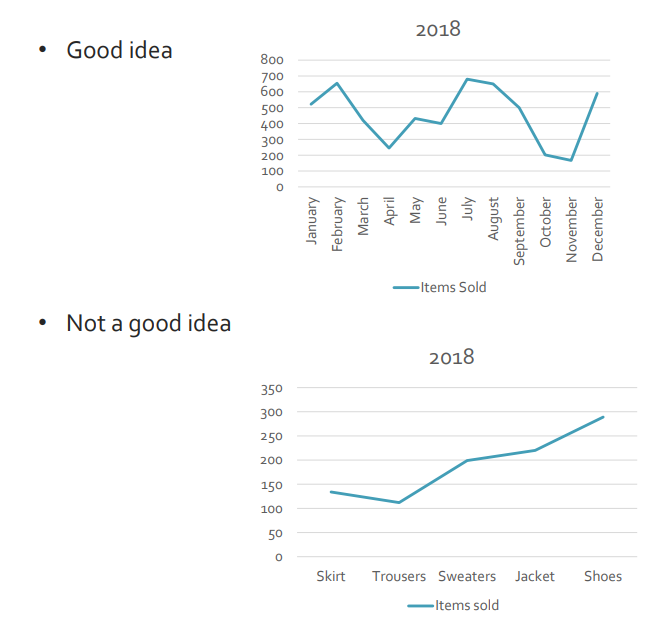
\includegraphics[width=0.5\textwidth]{images/BarCharts.png} 
    \caption{Bar Charts}
    \label{fig:immagine}
\end{figure}
\subsubsection{Histograms}
Frequenza degli elementi. Dati bivariati: una variabile indipendente quantizzata in intervalli 
(blocchi) e una variabile dipendente.
\begin{figure}[H]
    \centering
    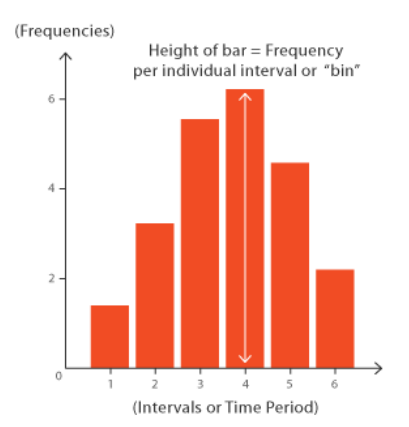
\includegraphics[width=0.5\textwidth]{images/Histograms.png} 
    \caption{Histograms}
    \label{fig:immagine}
\end{figure}
\subsubsection{Pie Charts}
Mostrare proporzioni e percentuali tra le categorie. Utile per dare un'idea rapida e confrontare una fetta rispetto al totale, non adatto per confronti accurati. Altri svantaggi: numero limitato di valori, 
occupazione dello spazio.
\begin{figure}[H]
    \centering
    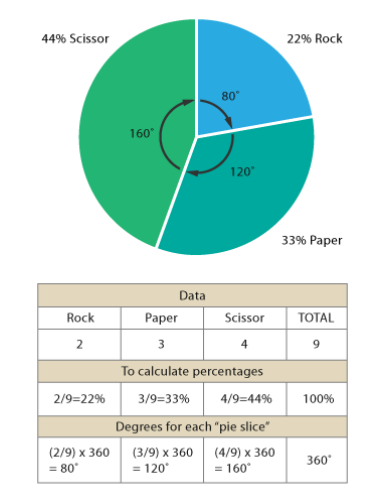
\includegraphics[width=0.5\textwidth]{images/PieChart.png} 
    \caption{Pie Charts}
    \label{fig:immagine}
\end{figure}

\subsubsection{Donut Charts}
Grafici a torta con l'area centrale tagliata. Maggiore enfasi sulla lunghezza dell'arco rispetto all'area. 
Più efficienti in termini di spazio.
\begin{figure}[H]
    \centering
    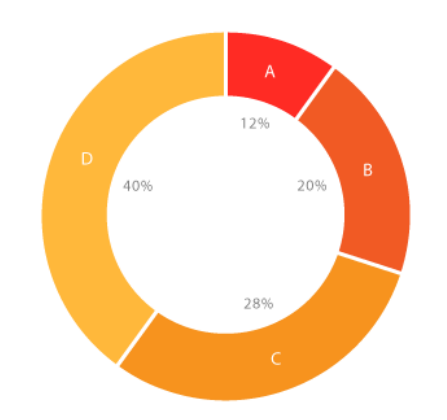
\includegraphics[width=0.5\textwidth]{images/DonutCharts.png} % Sostituisci 'nome_immagine' con il nome del tuo file immagine
    \caption{Donut Charts}
    \label{fig:immagine}
\end{figure}
\subsubsection{Scatter plots}
Relazione tra attributi: visualizzazione di come una quantità è correlata a un'altra 
(e analisi di cluster, valori anomali, ecc.). Dati bivariati: 
due attributi quantitativi indipendenti.
\begin{figure}[H]
    \centering
    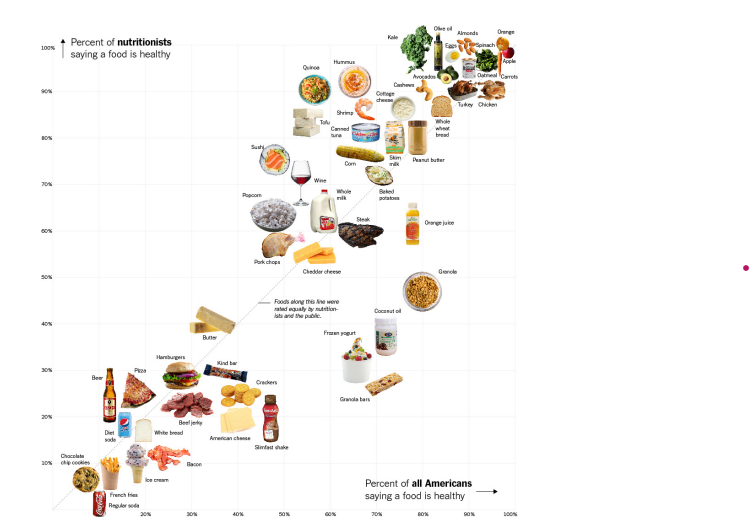
\includegraphics[width=0.5\textwidth]{images/ScatterPlots.png} % Sostituisci 'nome_immagine' con il nome del tuo file immagine
    \caption{Scatter plots}
    \label{fig:immagine}
\end{figure}
\subsubsection{Slope Charts}
Alternativa ai Scatter plots: assi paralleli, ogni elemento è una linea che collega due quantità.
\begin{figure}[H]
    \centering
    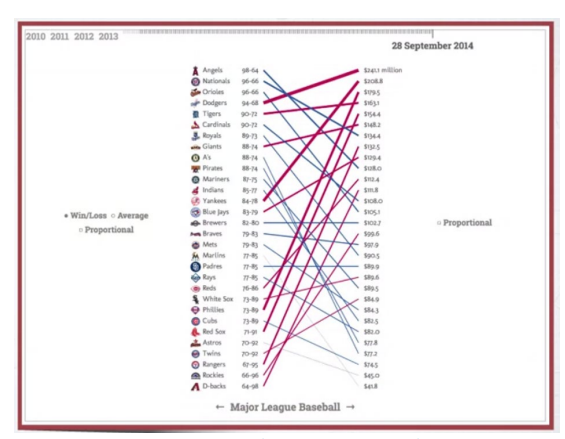
\includegraphics[width=0.5\textwidth]{images/SlopeCharts.png} 
    \caption{Slope Charts}
    \label{fig:immagine}
\end{figure}
\subsubsection{Line Charts}
\begin{figure}[H]
    \centering
    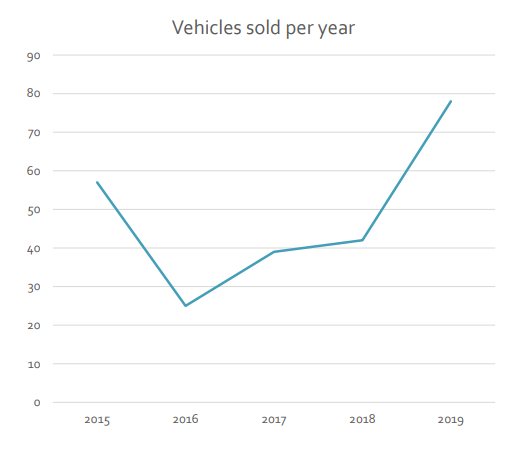
\includegraphics[width=0.5\textwidth]{images/LineCharts.png}
    \caption{Line Charts}
    \label{fig:immagine}
\end{figure}
\subsubsection{Area Charts}
Line Charts dove l'area sotto alla linea è riempita.
\begin{figure}[H]
    \centering
    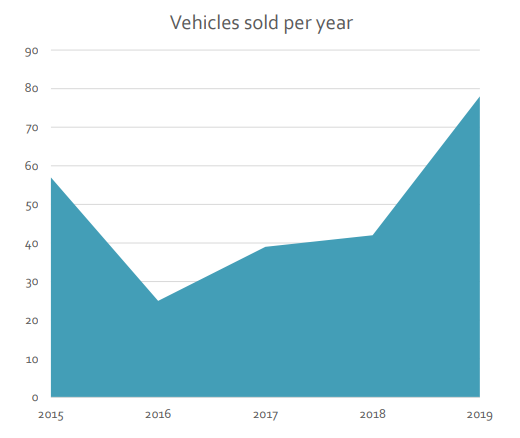
\includegraphics[width=0.5\textwidth]{images/AreaCharts.png}
    \caption{Area Charts}
    \label{fig:immagine}
\end{figure}
\subsubsection{Chropleth maps}
Come si distribuisce una quantità nelle diverse aree/geografiche/regioni. Colori, sfumature, pattern sono utilizzati per rappresentare la quantità associata alle aree/regioni. Buona panoramica (ma non confronto accurato). Rischio: 
confondere l'area geografica con i valori dei dati (prestare attenzione alla normalizzazione).
\begin{figure}[H]
    \centering
    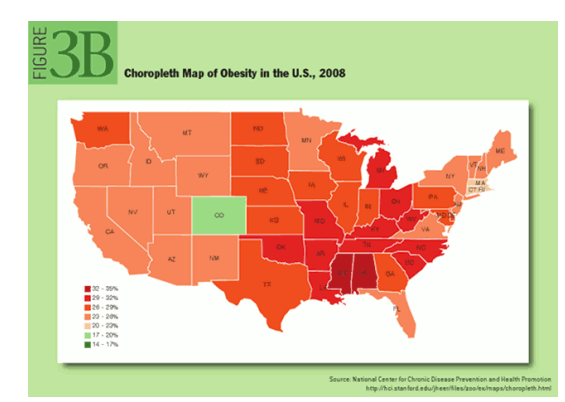
\includegraphics[width=0.5\textwidth]{images/Chropolet.png} 
    \caption{Chropleth maps}
    \label{fig:immagine}
\end{figure}
\subsubsection{Symbol maps}
Come si distribuisce una quantità lungo due coordinate spaziali. Un simbolo (spesso un disco o un quadrato) è posizionato 
in un punto e dimensionato in modo che la sua area sia proporzionale alla quantità associata al punto.
\begin{figure}[H]
    \centering
    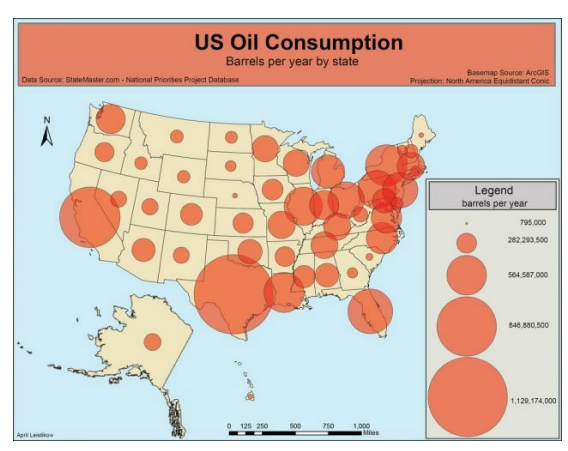
\includegraphics[width=0.5\textwidth]{images/SymbolMaps.png} 
    \caption{Symbol maps}
    \label{fig:immagine}
\end{figure}

\subsection{Grafici Fondamentali (Attributi Multipli)}
\subsubsection{Stacked Bar Charts}
\begin{figure}[H]
    \centering
    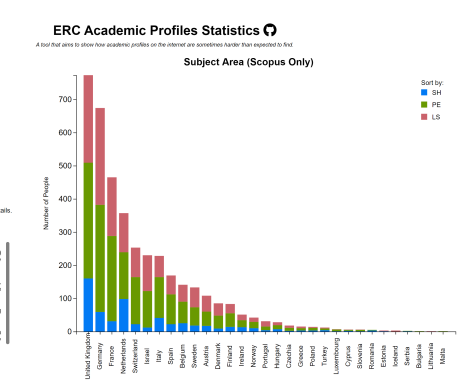
\includegraphics[width=0.5\textwidth]{images/StackedBar.png} % Sostituisci 'nome_immagine' con il nome del tuo file immagine
    \caption{Stacked Bar Charts}
    \label{fig:immagine}
\end{figure}
\subsubsection{Grouped Bar Charts}
\begin{figure}[H]
    \centering
    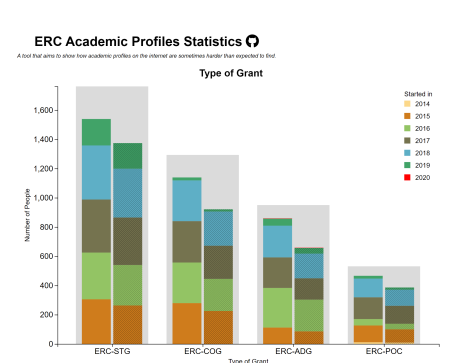
\includegraphics[width=0.5\textwidth]{images/GroupedBar.png} % Sostituisci 'nome_immagine' con il nome del tuo file immagine
    \caption{Grouped Bar Charts}
    \label{fig:immagine}
\end{figure}
\subsubsection{Stacked Line Charts}
\begin{figure}[H]
    \centering
    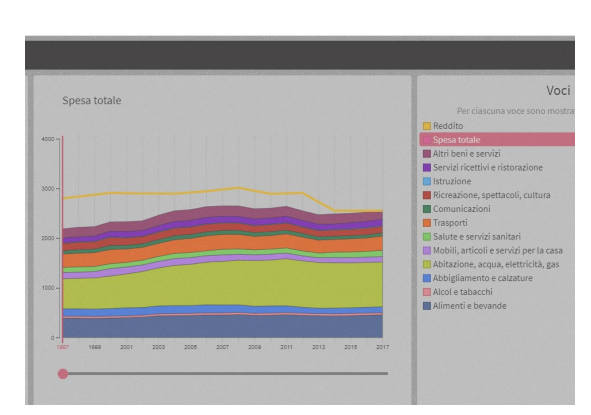
\includegraphics[width=0.5\textwidth]{images/Stacked.png} % Sostituisci 'nome_immagine' con il nome del tuo file immagine
    \caption{Stacked Line Charts}
    \label{fig:immagine}
\end{figure}
\subsubsection{Line Charts Series}
\begin{figure}[H]
    \centering
    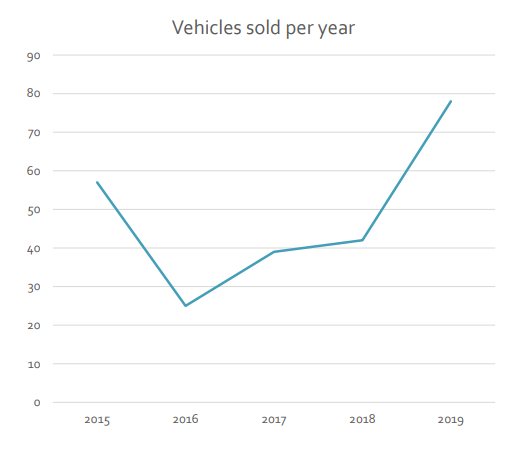
\includegraphics[width=0.5\textwidth]{images/LineCharts.png} % Sostituisci 'nome_immagine' con il nome del tuo file immagine
    \caption{Line Charts Series}
    \label{fig:immagine}
\end{figure}
\subsubsection{Bubble Charts}
\begin{figure}[H]
    \centering
    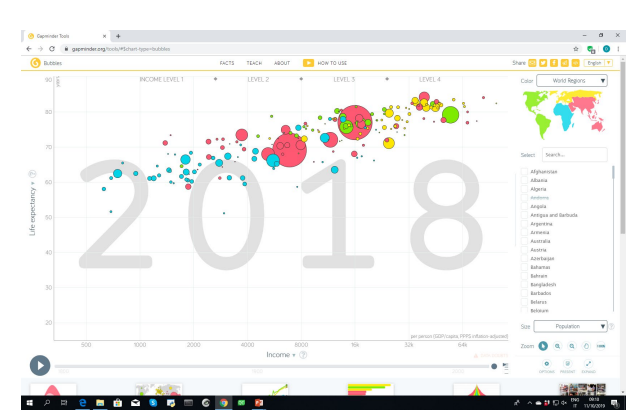
\includegraphics[width=0.5\textwidth]{images/Bubble.png} % Sostituisci 'nome_immagine' con il nome del tuo file immagine
    \caption{Bubble Charts}
    \label{fig:immagine}
\end{figure}
\subsubsection{Small multiples}
\begin{figure}[H]
    \centering
    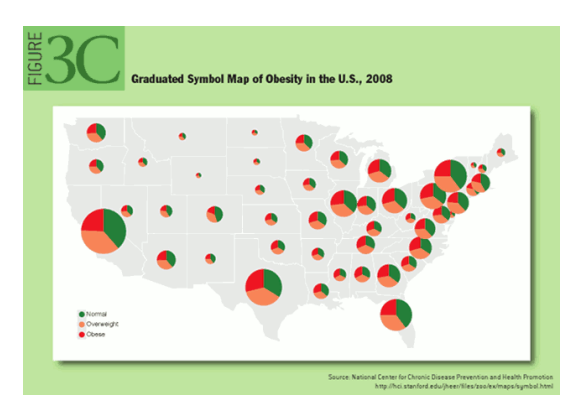
\includegraphics[width=0.5\textwidth]{images/SmallMultiples2.png} % Sostituisci 'nome_immagine' con il nome del tuo file immagine
    \caption{Small multiples}
    \label{fig:immagine}
\end{figure}
\subsubsection{Symbol Maps}
\begin{figure}[H]
    \centering
    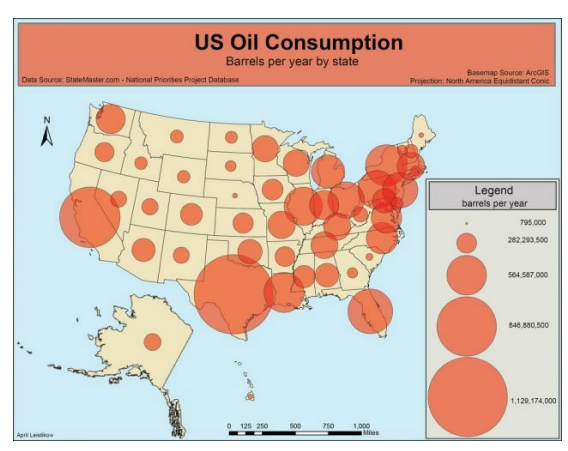
\includegraphics[width=0.5\textwidth]{images/SymbolMaps.png} % Sostituisci 'nome_immagine' con il nome del tuo file immagine
    \caption{Symbol Maps}
    \label{fig:immagine}
\end{figure}
\subsection{Grafici Fondamentali (Attributi Gerarchici)}
\subsubsection{Sunburst Charts}
\begin{figure}[H]
    \centering
    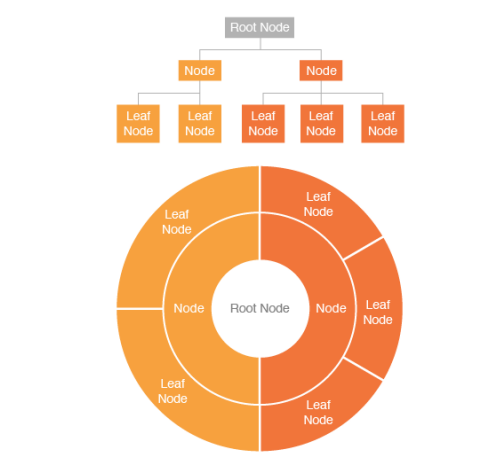
\includegraphics[width=0.5\textwidth]{images/SunBurst.png} % Sostituisci 'nome_immagine' con il nome del tuo file immagine
    \caption{Sunburst Charts}
    \label{fig:immagine}
\end{figure}
\subsubsection{Treempas}
\begin{figure}[H]
    \centering
    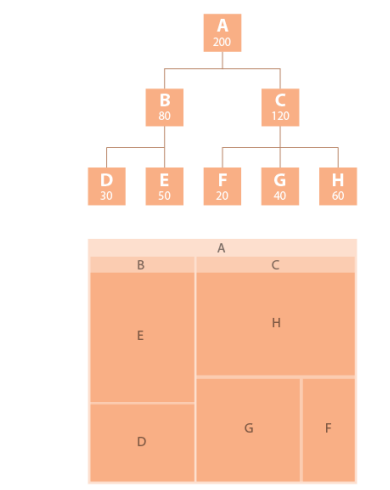
\includegraphics[width=0.5\textwidth]{images/TreeMpas.png} % Sostituisci 'nome_immagine' con il nome del tuo file immagine
    \caption{Treempas}
    \label{fig:immagine}
\end{figure}
\section{Information Visualization II}
\subsection{Visual Encoding}
Le visualizzazioni sono composte da \textbf{marks} (segnali) e 
\textbf{channels} (canali). I marks sono gli oggetti grafici che rappresentano gli elementi di dati (ad esempio, punti, linee, barre).
I channels sono le proprietà grafiche che rappresentano gli attributi dei dati (ad esempio, colore, posizione, forma, dimensione).


La codifica visiva significa passare dai dati alle rappresentazioni visive.
La codifica richiede non solo la scelta di un grafico appropriato per i dati in questione (tipo e semantica),
ma anche la selezione degli elementi grafici individuali e delle loro proprietà.

\subsection{Graphical Elements}
\begin{figure}[H]
    \centering
    \begin{minipage}{0.45\textwidth}
        \centering
        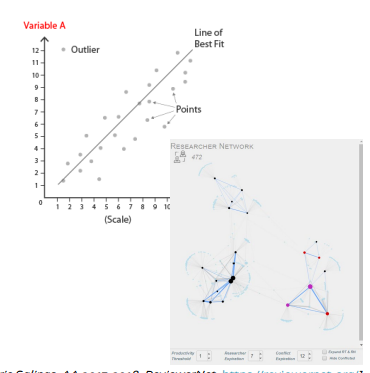
\includegraphics[width=\linewidth]{images/Marks.png} 
        \caption{Esempio di Marks}
        \label{fig:immagine1}
    \end{minipage}\hfill
    \begin{minipage}{0.45\textwidth}
        \centering
        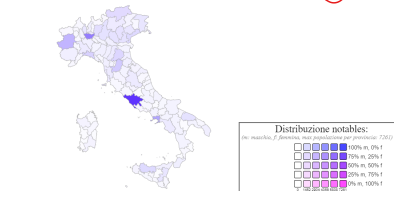
\includegraphics[width=\linewidth]{images/Channels.png} % Sostituisci 'immagine2' con il nome del tuo file immagine
        \caption{Esempio di Channels}
        \label{fig:immagine2}
    \end{minipage}
\end{figure}
Le componenti contestuali sono elementi che rendono più semplice interpretare le visualizzazioni.
Un esempio sono: le labesls, annotazioni, legende, griglie, assi cartesiani.
\begin{figure}[H]
    \centering
    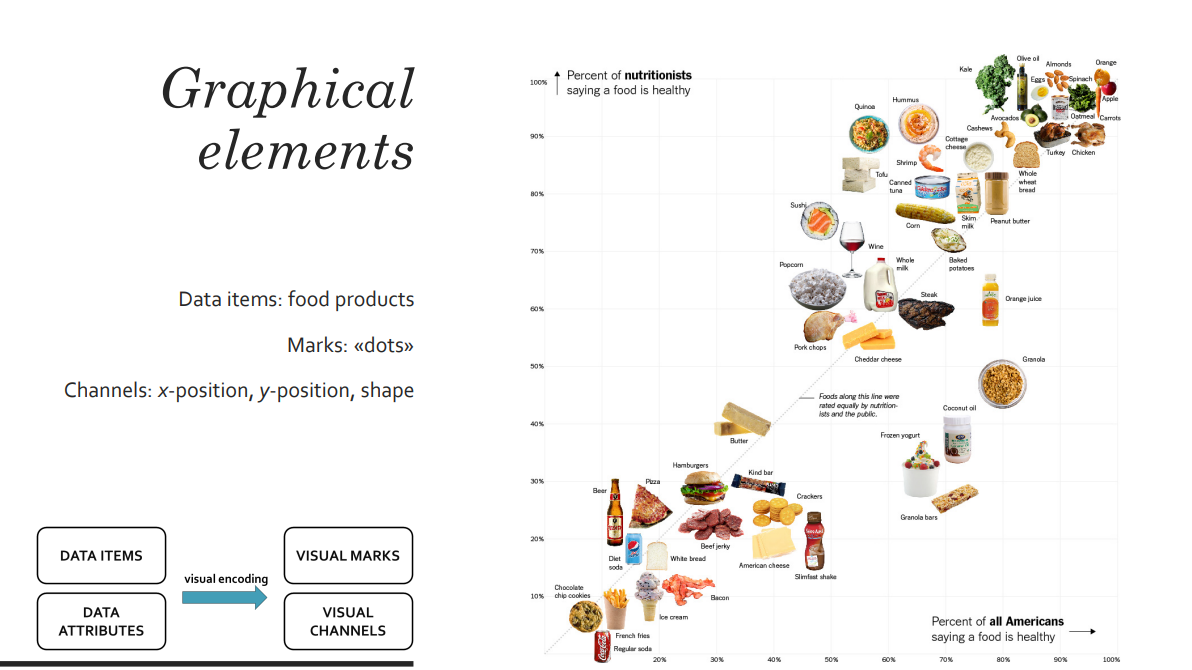
\includegraphics[width=0.5\textwidth]{images/CompleteExMC.png} % Sostituisci 'nome_immagine' con il nome del tuo file immagine
    \caption{Esempio completo di Channels e Marks di un grafico}
    \label{fig:immagine}
\end{figure}
\subsection{Visual decoding}
\begin{figure}[H]
    \centering
    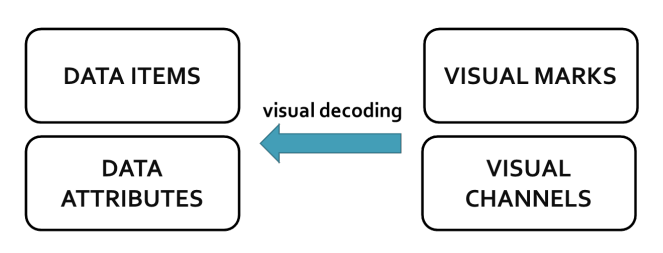
\includegraphics[width=0.5\textwidth]{images/VisDec.png} % Sostituisci 'nome_immagine' con il nome del tuo file immagine
    \caption{Visual Decoding}
    \label{fig:immagine}
\end{figure}
Per \textbf{Visual Decoding} si intende destrutturare una rappresentazione visiva nei suoi principali elementi e identificare:
\begin{itemize}
    \item gli elementi grafici, quali sono i segnali visivi? Quali sono i canali visivi?
    \item le regole di mappatura (ossia, le informazioni che i singoli elementi grafici rappresentano)
        quali elementi di dati rappresentano i segnali? Quali attributi rappresentano i canali?
\end{itemize}
È utile per valutare e ridisegnare le visualizzazioni.

\begin{figure}[H]
    \centering
    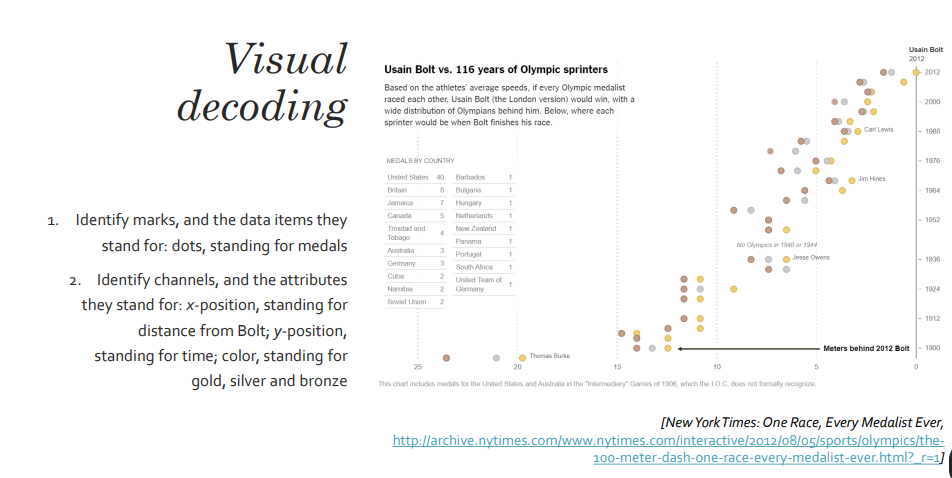
\includegraphics[width=0.5\textwidth]{images/ExComplDec.png} % Sostituisci 'nome_immagine' con il nome del tuo file immagine
    \caption{Esempio completo di Decoding}
    \label{fig:immagine}
\end{figure}

\subsubsection{Quality Evaluation}
La valutazione di una visualizzazione può basarsi su due principi 
guida principali: \textbf{Expressiveness} ed \textbf{Effectiveness}.
\textbf{Expressiveness}: la Visual representation dovrebbe rappresentare tutte e solo le relazioni che esistono nei dati.
Le informazioni rilevanti dovrebbero essere prioritarie e quindi codificate con i canali più efficaci/accurati.
\begin{figure}[H]
    \centering
    \begin{minipage}{0.45\textwidth}
        \centering
        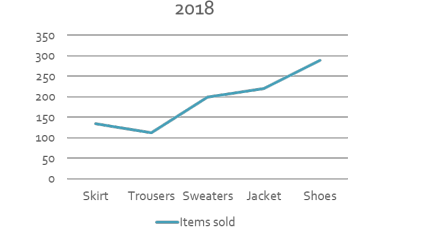
\includegraphics[width=\linewidth]{images/ErroreEff.png} 
        \caption{Dati non ordinati che sembrano ordinati (nell'esempio seguente, stiamo mostrando informazioni su un trend che non è nei dati:
         la forma della linea non ha significato).}
        \label{fig:immagine1}
    \end{minipage}\hfill
    \begin{minipage}{0.45\textwidth}
        \centering
        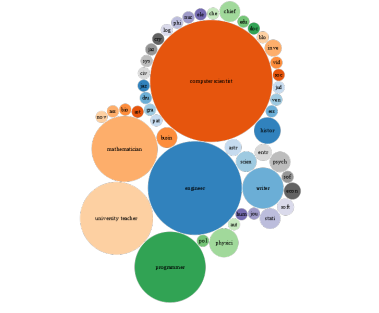
\includegraphics[width=\linewidth]{images/ErroreEff2.png} % Sostituisci 'immagine2' con il nome del tuo file immagine
        \caption{utilizzo dei colori quando non restituiscono alcuna informazione}
        \label{fig:immagine2}
    \end{minipage}
\end{figure}
\subsubsection{Percentuale di Accuracy}
Quanto sono efficaci i canali nel trasmettere diversi tipi di attributi?
Uno dei (possibili) riassunti per attributi quantitativi.
\begin{figure}[H]
    \centering
    \begin{minipage}{0.45\textwidth}
        \centering
        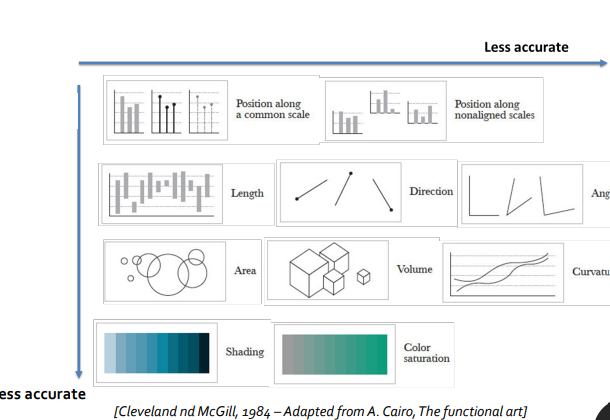
\includegraphics[width=\linewidth]{images/percentAcc1.png} 
        \caption{Riassunto dell'accuracy di ogni grafico.}
        \label{fig:immagine1}
    \end{minipage}\hfill
    \begin{minipage}{0.45\textwidth}
        \centering
        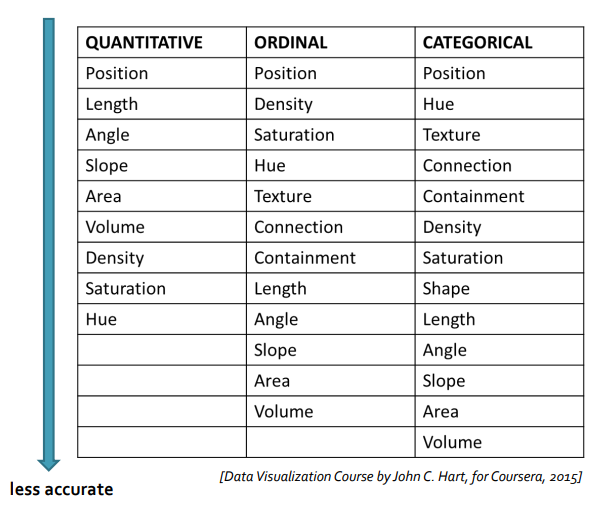
\includegraphics[width=\linewidth]{images/percentAcc2.png} 
        \caption{Riassunto dell'accuracy di ogni grafico}
        \label{fig:immagine2}
    \end{minipage}
\end{figure}
\subsection{Altri tipi di grafici}
\subsubsection{WordClouds}
Rappresentazione di quanto frequentemente le parole appaiono in un determinato corpo di testo attraverso la dimensione della parola
Variazioni nell'arrangiamento e nel colore
Principalmente utilizzato per motivi estetici.
\begin{figure}[H]
    \centering
    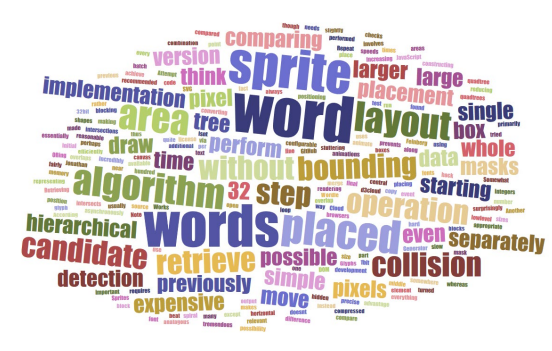
\includegraphics[width=0.5\textwidth]{images/WordClouds.png} 
    \caption{WordClouds}
    \label{fig:immagine}
\end{figure}
\subsubsection{Calligrams}
Testi disposti in modo tale da formare un'immagine tematicamente correlata.
L'immagine creata dalle parole illustra il testo esprimendo visivamente qualcosa associato (o in contrasto) a ciò che il testo dice.
\begin{figure}[H]
    \centering
    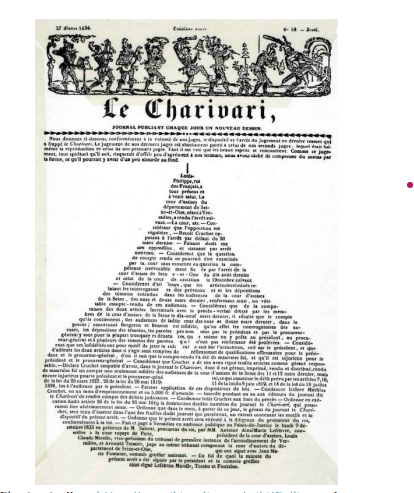
\includegraphics[width=0.5\textwidth]{images/Calligrams.png} 
    \caption{Calligrams}
    \label{fig:immagine}
\end{figure}

\subsubsection{Flow Maps}

Raffigurare il movimento delle entità posizionando linee tracciate sopra delle mappe (spazio e tempo)
Lo spessore, il colore, ecc. possono codificare informazioni aggiuntive
In questa mappa: dimensioni delle truppe, distanza percorsa, temperatura, latitudine e longitudine, direzione del viaggio, tempo.
\begin{figure}[H]
    \centering
    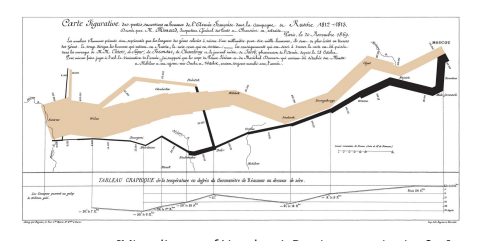
\includegraphics[width=0.5\textwidth]{images/FlowMaps.png}
    \caption{Flow Maps}
    \label{fig:immagine}
\end{figure}
\subsubsection{Chernoff faces}
Ragionamento: siamo molto bravi nel riconoscere i volti.
Introdotto da Herman Chernoff nel 1973
Variabili sono mappate su tratti del viso
(larghezza/curvatura della bocca, dimensione verticale del viso, dimensione/inclinazione/separazione degli occhi, dimensione delle sopracciglia, posizione verticale delle sopracciglia…)
\begin{figure}[H]
    \centering
    \includegraphics[width=0.5\textwidth]{images/Chernofffaces.png} 
    \caption{Chernoff faces}
    \label{fig:immagine}
\end{figure}
\subsubsection{Multidimensional Icons}
Spence e Parr (1991) proposero di codificare le proprietà di un oggetto in una semplice rappresentazione tramite icone. 
Hanno applicato questo approccio per verificare le offerte di permanenza.
\begin{figure}[H]
    \centering
    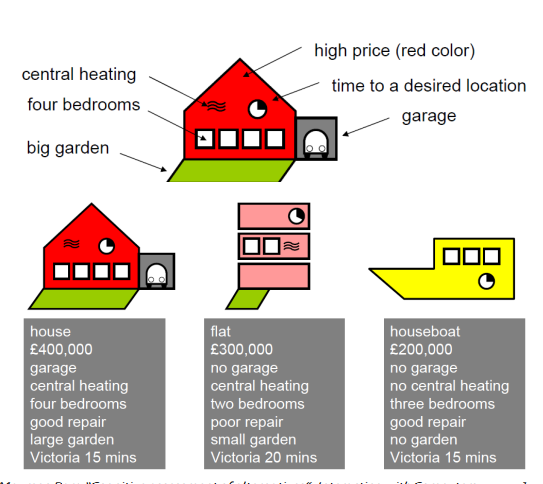
\includegraphics[width=0.5\textwidth]{images/MultiIcon.png} 
    \caption{Multidimensional Icons}
    \label{fig:immagine}
\end{figure}
\subsubsection{Petal as a gliph}
L'idea di Moritz Stefaner per visualizzare un indice di vita consiste nel mappare diverse variabili (relative alle condizioni di vita materiale e alla qualità della vita) in petali di diverse dimensioni, per confrontare il benessere tra paesi.
\begin{figure}[H]
    \centering
    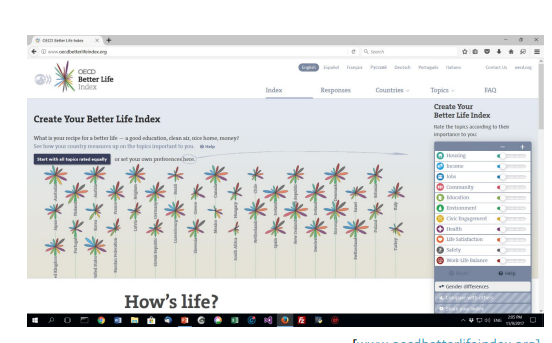
\includegraphics[width=0.5\textwidth]{images/PetalGliph.png} 
    \caption{Petal as a gliph}
    \label{fig:immagine}
\end{figure}


\section{Applied Perception}
Abbiamo visto che la visualizzazione delle informazioni consiste nel trasformare i dati in una rappresentazione 
visuale in modo che un essere umano possa estrarre informazioni utili da essi.
L'\textbf{Effectiveness} di una rappresentazione visuale non è arbitraria: ma dipende fortemente su come funziona il cervello.
Remind: l'efficacia si riferisce alla capacità di una rappresentazione visiva, come un grafico, una mappa o un diagramma, di comunicare in modo chiaro e comprensibile le informazioni desiderate. 
Capire come funziona la percezione può aiutare a prendere decisioni informate riguardo ai design delle visualizzazioni.
L'occhio umano svolge un ruolo fondamentale nella percezione visiva, essendo il principale organo sensoriale che ci consente di interpretare il mondo circostante.
L'\textbf{acuità visiva} è una misura della capacità dell'occhio di distinguere dettagli fini e di percepire chiaramente gli oggetti.
Viene spesso misurata in termini di precisione nella lettura di lettere o simboli su una tavola ottotipica posta a una certa distanza.
La nostra percezione è sensibile al contrasto di pattern, alla frequenza e all'orientamento. Inoltre, il colore influisce sulla funzione del sistema di contrasto spaziale (CSF).
Il visual Cortex è una parte del cervello che gestisce l'elaborazione delle informazioni visive provenienti dagli occhi.
\begin{figure}[H]
    \centering
    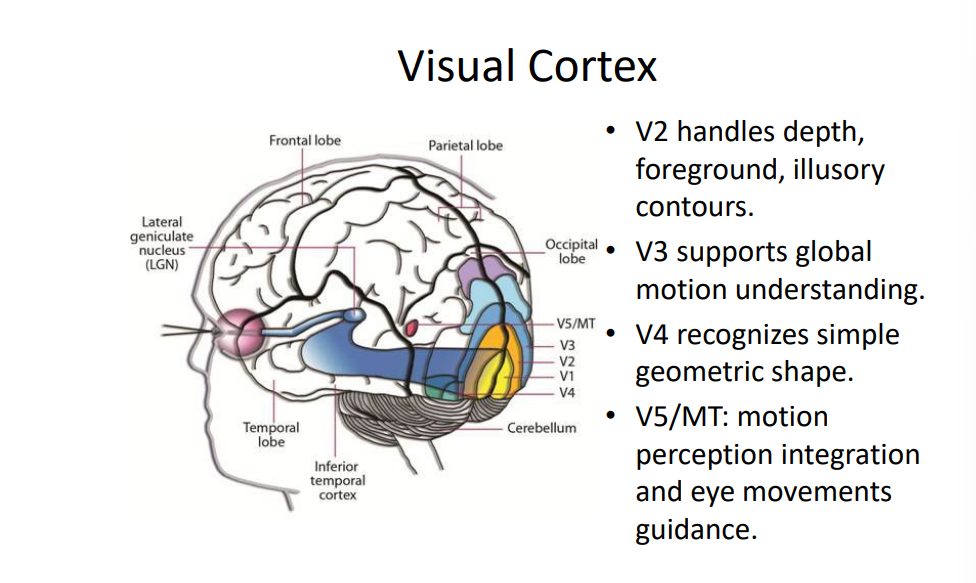
\includegraphics[width=0.5\textwidth]{images/VisualCortex.png} 
    \caption{Divisione del cervello}
    \label{fig:immagine}
\end{figure}
\subsection{Illusions}
Il campo recettivo di una cellula è l'area visiva sulla quale una cellula risponde alla luce.
Le cellule gangliari della retina sono organizzate con campi recettivi circolari.
Quando vengono stimolate al centro, vengono eccitate; quando vengono stimolate al di fuori del centro, vengono inibite.
\subsubsection{Mach Banding}
Le "Mach bands" (bande di Mach) sono un fenomeno ottico che si verifica quando si osservano transizioni tra regioni di luce e ombra su una superficie, creando 
percezioni di contrasto accentuato lungo i confini.
\begin{figure}[H]
    \centering
    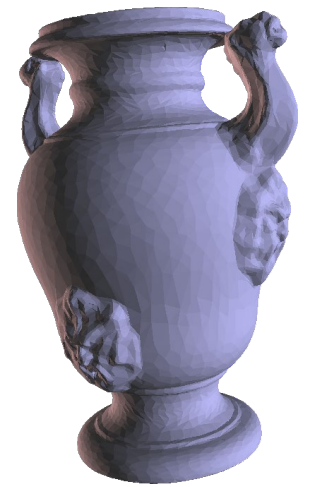
\includegraphics[width=0.5\textwidth]{images/MachBand.png} 
    \caption{Mach Banding}
    \label{fig:immagine}
\end{figure}
\subsubsection{Hermann Grid illusions}

La griglia di Hermann è un'illusione ottica che mette in evidenza l'interazione tra le cellule retiniche e il modo in cui il cervello elabora le informazioni visive. Questa illusione è composta da una griglia di linee grigie disposte a intervalli regolari, 
con dei punti neri posizionati strategicamente agli incroci delle linee.
Si ritiene che l'illusione sia causata dalla percezione del contrasto e dall'inibizione laterale nel sistema visivo. Le cellule retiniche inviano segnali al cervello che possono essere interpretati in modo errato, 
facendo percepire punti ombrosi o grigi nei punti di intersezione delle linee.
\begin{figure}[H]
    \centering
    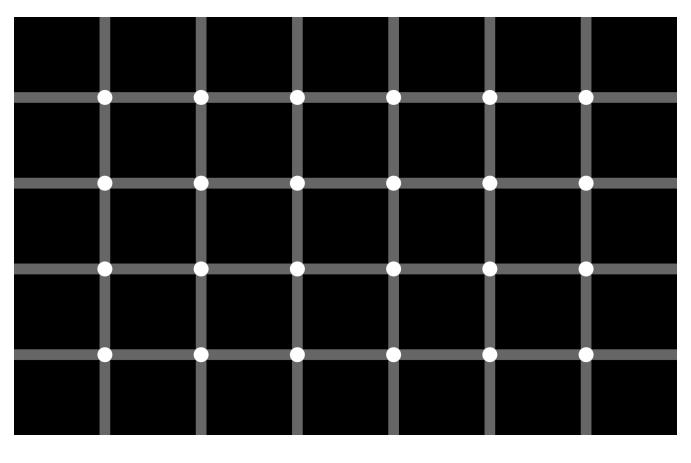
\includegraphics[width=0.5\textwidth]{images/HermmanG.png} 
    \caption{Divisione del cervello}
    \label{fig:immagine}
\end{figure}
\subsubsection{Chevreul Illusion}

L'illusione di Chevreul, chiamata anche illusione dei contrasti simultanei, è un fenomeno ottico che coinvolge la percezione del colore. Questa illusione è dovuta alla sensibilità del nostro sistema visivo ai contrasti e alla relativa interpretazione dei colori circostanti.
Nell'illusione di Chevreul, se viene disegnata una serie di linee parallele in tonalità di grigio simile su uno sfondo bianco, la percezione visiva può far sembrare che i toni di grigio varino lungo le linee. Questo accade a causa dell'interazione tra i colori circostanti e la nostra percezione del contrasto.
Se due tonalità di grigio simili sono separate da una riga più chiara, il grigio sembrerà più scuro del suo vero colore. Al contrario, se sono separate da una riga più scura, sembrerà più chiaro. Questo effetto può far sembrare che i toni di grigio cambino o che vi sia un gradiente lungo le linee parallele,
quando in realtà la differenza di colore non esiste realmente.
 \begin{figure}[H]
    \centering
    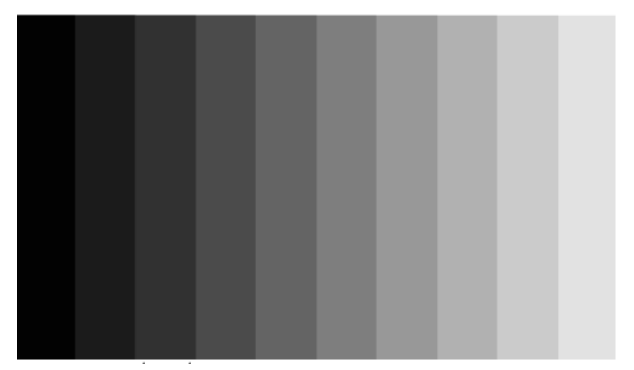
\includegraphics[width=0.5\textwidth]{images/Chevr.png} 
    \caption{Chevreul illusion}
    \label{fig:immagine}
\end{figure}
 \subsubsection{Greyscale Maps}
Questi effetti visivi possono portare a grandi errori quando si leggono informazioni quantitative visualizzate utilizzando una mappa in scala di grigi.
Utilizzare mappe in scala di grigi per rappresentare pochi valori (!)
\subsubsection{The Cornsweet Effect}
Le illusioni di Cornsweet sono un tipo di illusione ottica che evidenzia la percezione umana del contrasto e dei confini tra diverse superfici o tonalità. Questo tipo di illusione si basa sul modo in cui il cervello elabora i cambiamenti graduali di luminosità o colore.
Nell'illusione di Cornsweet, due aree contigue hanno un confine graduale tra loro e una transizione graduale di luminosità o colore. Nonostante la transizione sia graduale e non ci sia un cambiamento netto, la percezione visiva può far 
sembrare che ci sia un confine più netto o un cambiamento repentino.
\begin{figure}[H]
    \centering
    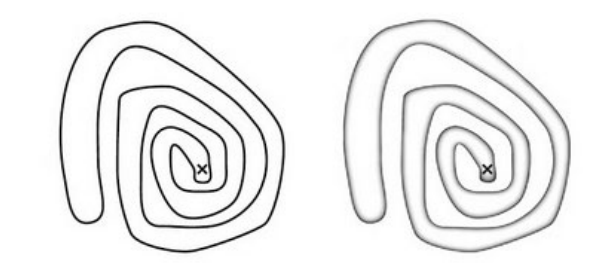
\includegraphics[width=0.5\textwidth]{images/Cornsweet.png} 
    \caption{Cornsweet Effect}
    \label{fig:immagine}
\end{figure}
L'effetto Cornsweet può essere utilizzato per evidenziare regioni delimitate.
Parlando dell'utilizzo delle scale di grigi, in sostanza ci sono delle regole da seguire:
Non utilizzare per mappe o per confrontare molti valori.
Utilizzare per evidenziare:
\begin{itemize}
    \item Regioni delimitate
    \item Elementi importanti (riducendo il contrasto luminoso degli elementi non importanti)
    \item Regolare la luminanza dello sfondo per ottenere una migliore leggibilità.
\end{itemize}
\subsection{Eye Movements}
\textbf{Movimenti oculari:}
\begin{itemize}
    \item \textbf{Movimenti saccadici}: movimenti balistici degli occhi che cambiano il punto di fissazione. Possono essere volontari o scatenati da stimoli.
    \item \textbf{Movimenti di inseguimento lento}: movimenti lenti degli occhi per mantenere uno stimolo in movimento sulla fovea.
    \item \textbf{Movimenti di vergenza}: allineano la fovea di ciascun occhio a un bersaglio in base alla sua distanza.
    \item \textbf{Movimenti vestibolo-oculari}: stabilizzano gli occhi compensando i movimenti della testa.

\end{itemize}
\subsubsection{Preattentive Processes}

I processi preattentivi si riferiscono a quelle operazioni cognitive che avvengono automaticamente e
 istantaneamente nell'elaborazione delle informazioni sensoriali prima che una persona focalizzi la sua attenzione in modo consapevole su di esse. 
 Questi processi avvengono in modo rapido e automatico, senza richiedere uno sforzo cosciente.
Sono responsabili della capacità del cervello di elaborare estrarre informazioni visive, uditiva o tattili in modo veloce ed efficiente. Questi processi sono fondamentali nell'organizzazione delle informazioni sensoriali e possono avvenire a livelli inconsci della percezione umana.
Caratteristiche visive elaborate preattivamente:
\begin{itemize}
    \item Orientamento ; Curvatura ; Forma ; Dimensione ; Colore ;
    Luce/Ombra ; Contenimento ; Concavità/Convessità ;
    \item Alcune di queste non sono simmetriche.
        Caratteristiche visive non elaborate preattivamente:
        Giunzione ; Parallelismo
\end{itemize}
Alcuni processi preattentivi non sono simmetrici:
Aggiungere segni è più efficiente che rimuovere segni.
Aumentare la nitidezza è più efficiente che diminuire la nitidezza.
Un oggetto grande circondato da oggetti piccoli è più efficiente di un oggetto piccolo circondato da oggetti grandi.

\subsubsection{Gestalt Laws}
Le leggi della Gestalt sono principi fondamentali della psicologia della percezione che descrivono come il cervello umano organizza e interpreta le informazioni sensoriali 
per creare una percezione significativa e coerente del mondo che ci circonda. 
\begin{enumerate}
    \item \textbf{Legge della Prossimità}: Gli oggetti vicini tra loro tendono ad essere visti come parte di un insieme o di un gruppo.
    
    \item \textbf{Legge della Similarità}: Gli elementi simili per forma, colore, dimensione o altre caratteristiche tendono ad essere raggruppati insieme nella percezione.
    
    \item \textbf{Legge della Connessione}: Gli oggetti connessi sono percepiti come correlati.
        Collegare diversi oggetti con una linea è un modo efficace per esprimere che esiste una relazione tra di essi.
    
    \item \textbf{Legge della Continuità}: Gli oggetti posti lungo una linea o una curva tendono ad essere visti come parte di un modello o di un flusso continuo.
    
    \item \textbf{Legge della Simmetria}: Gli oggetti disposti simmetricamente sono percepiti come formare un insieme visivo anziché essere considerati entità separate.
     La simmetria è meglio percepita per gli assi orizzontali e verticali.
    
    \item \textbf{Legge della Chiusura}: Le persone tendono a percepire le figure incomplete come forme complete riempiendo le parti mancanti.
    
    \item \textbf{Legge della Simplicità o della Buona Forma}: La percezione tende a organizzare gli stimoli in modo da formare figure semplici e coerenti piuttosto che configurazioni disordinate o complesse.
    
    \item \textbf{Legge della Destinzione Figure-Ground}: Gli oggetti possono essere percepiti come figure distinte rispetto al loro sfondo circostante.
    
    \item \textbf{Legge del Movimento Comune}: Gli oggetti che si muovono nella stessa direzione o seguendo lo stesso modello di movimento possono essere percepiti come parte di un unico oggetto o gruppo.
  \end{enumerate}
  \subsection{Illusions}
  \subsubsection{Muller-Lyer}
  \begin{figure}[H]
    \centering
    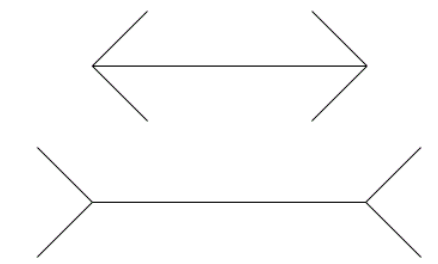
\includegraphics[width=0.5\textwidth]{images/Muller.png} 
    \caption{Muller-Lyer Illusions}
    \label{fig:immagine}
\end{figure}
  Queste due linee hanno lunghezze uguali ma vengono percepite di lunghezze diverse.
    \begin{itemize}
        \item Due spiegazioni:
        \begin{enumerate}
            \item Spiegazione prospettica
            \item Spiegazione del baricentro
        \end{enumerate}
    \end{itemize}
  \subsubsection{Wundt}
  Queste illusioni coinvolgono principalmente la percezione delle dimensioni, delle proporzioni e delle distanze tra gli oggetti, portando
   a percezioni distorte o erronee della realtà visiva.
   \begin{figure}[H]
    \centering
    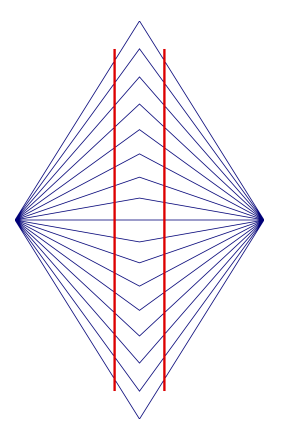
\includegraphics[width=0.5\textwidth]{images/Wundt.png} 
    \caption{Muller-Lyer Illusions}
    \label{fig:immagine}
\end{figure}
  \subsubsection{Hering}
  Un'altra illusione simile (effetto invertito dell'illusione di Wundt).
\begin{itemize}
    \item Possibili spiegazioni:
    \begin{enumerate}
        \item Inibizione laterale
        \item Effetto prospettico
        \item Ritardi temporali nell'elaborazione visiva
    \end{enumerate}
\end{itemize}

  \subsubsection{Horizontal–Vertical Illusion}
  \begin{figure}[H]
    \centering
    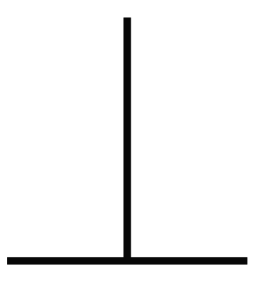
\includegraphics[width=0.5\textwidth]{images/HorizontalVertical.png} 
    \caption{Horizontal–Vertical Illusion}
    \label{fig:immagine}
\end{figure}
  Un'altra semplice illusione scoperta da Wundt.
  La linea verticale viene percepita come lunga al 30\% in più rispetto alla linea orizzontale.
  Sono state osservate differenze (piccole) tra le culture.
  Questo vale anche per le linee che si intersecano.
  \subsubsection{Comparing Area}
  Confrontare le aree è difficile (ricordare le aree dei cerchi appena menzionate).
  \begin{figure}[H]
    \centering
    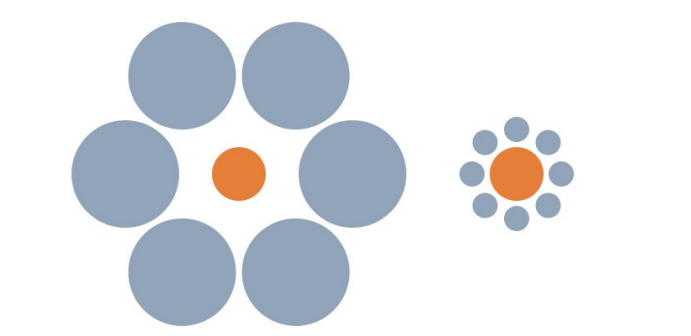
\includegraphics[width=0.5\textwidth]{images/Comparing.png} 
    \caption{Comparing Area}
    \label{fig:immagine}
\end{figure} 
    \begin{itemize}
        \item Quando confrontiamo le aree, le proporzioni sono sottovalutate (peggio per i volumi).
        \item Flannery (1970) propose di compensare la percezione applicando un fattore di scala percettiva.
        \item Tufte, nel suo famoso libro "The Visual Display of Quantitative Information" (2001), si oppose a qualsiasi cosa tranne che l'uso di una scala assoluta, ovvero esclude la compensazione per le mancanze percettive umane.
    \end{itemize}
    La scalatura percettiva potrebbe essere insufficiente. Le cose sono più complesse da un punto di vista percettivo
\subsubsection{Weber's Law}
Ernst Heinrich Weber (1795 1878) ha condotto studi sulla percezione degli stimoli fisici da parte dei sensi umani (visione, udito, gusto, tatto e olfatto).
Legge di Weber: \\
$ \frac{\Delta S}{S}=K $ \\

Legge di Weber:
\begin{itemize}
    \item La percezione dipende dallo stimolo iniziale.
    \item  I rapporti sono più importanti dei valori assoluti.
\end{itemize}


\section{Applied Perception II }
\subsection{Color Vision}
La \textit{Color Vision} può essere considerata come superflua nella vita moderna
Ma il colore comunque è estreamamente utile nella data visualization:
\begin{itemize}
    \item Mostrare i patterns
    \item Labeling
    \item Mettere in evidenza
\end{itemize}
\begin{figure}[H]
    \centering
    \begin{minipage}{0.45\textwidth}
        \centering
        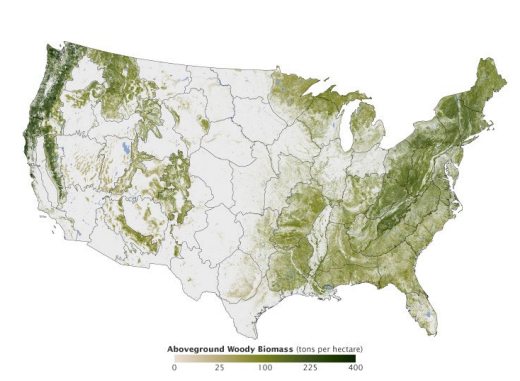
\includegraphics[width=\linewidth]{images/ColorVision.png} 
        \caption{Effetti della color vision}
        \label{fig:immagine1}
    \end{minipage}\hfill
    \begin{minipage}{0.45\textwidth}
        \centering
        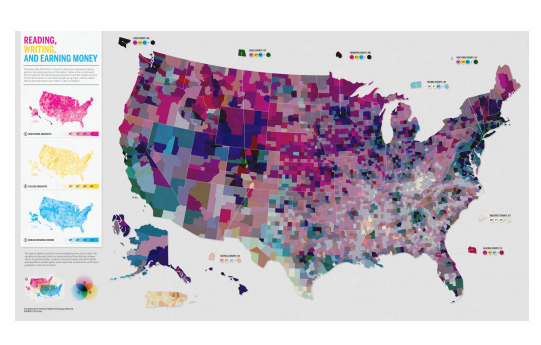
\includegraphics[width=\linewidth]{images/ColorVision2.png} 
        \caption{Effetti della color vision}
        \label{fig:immagine2}
    \end{minipage}
\end{figure}
Pensare al colore come un attributo di un oggetto invece che ad una caratteristica primaria(C.Ware).
\subsection{Trichromacy and Opponent process theories}
Abbbiamo, sulla retina, tre distinti recettori per i colori:
\begin{itemize}
    \item the \textbf{cones}: che sono attivi ai livelli normali di luce
    \item the \textbf{rods}: l'influenza dei rods sulla percezione può essere ignorata.
\end{itemize}
\subsubsection{Trichromacy theory}
I \textit{cones} sono sensibili alle diverse onde di luce.
Quindi, assorbono luce attorno lo spettro del colore blue, verde e rosso.
La teoria dice che percepiamo il colore tramite un sistema a tre canali.
Tutti gli spazi dei colori, anche se progettati per scopi diversi, sono tridimensionali.
\begin{figure}[H]
    \centering
    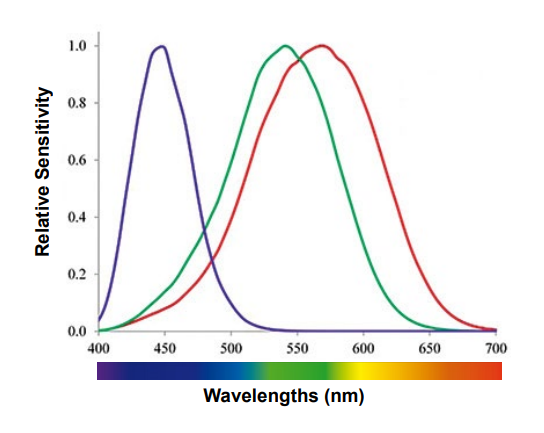
\includegraphics[width=0.5\textwidth]{images/Thrichromacy.png} 
    \caption{Trichromacy theory}
    \label{fig:immagine}
\end{figure}
\subsubsection{colour measurement and specifcation}
Dato che solo tre diversi recettori sono coinvolti nella colori vision, è possibile fare il match dei colori
usando un mix di tre colori, chiamati primari.
Dato uno standard di colori primari, si può usare una transformazione per creare lo stesso colore in output in device diversi 
\begin{figure}[H]
    \centering
    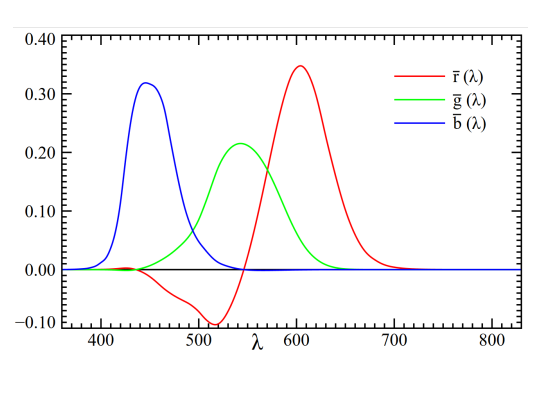
\includegraphics[width=0.5\textwidth]{images/RGB.png} 
    \caption{RGB color Matching Function}
    \label{fig:immagine}
\end{figure}
\subsubsection{CIE XYZ Color Space}

Lo spazio colore CIE XYZ è uno spazio colore standardizzato sviluppato dalla Commission Internationale de l'Eclairage (CIE). È un modello matematico che rappresenta tutti i colori visibili agli esseri umani attraverso tre valori numerici: X, Y e Z.
Questi valori sono definiti in base alle risposte dei tre tipi di coni presenti nell'occhio umano (sensibili alle lunghezze d'onda dei colori rosso, verde e blu).
Il valore Y rappresenta la luminosità, mentre X e Z descrivono la posizione orizzontale e verticale del colore nello spazio XYZ.
 
Il diagramma di cromaticità è uno strumento visivo utilizzato per rappresentare i colori visibili senza tener conto della luminosità. Questo diagramma rappresenta le proprietà del colore in termini di tonalità e saturazione, ignorando la luminanza.
\subsubsection{Opponent process theory}

Alla fine del XIX secolo, il psicologo tedesco Hering propose la teoria (successivamente supportata da prove sperimentali) secondo cui i coni della retina combinano il loro stimolo formando tre coppie di colori che competono tra loro per formare quello finale. Queste coppie, chiamate coppie antagoniste, sono: nero-bianco, giallo-verde e giallo-blu
\textbf{Evidenze a supporto della teoria:}
\begin{itemize}
  \item Nomenclatura
  \item Tonalità uniche
  \item Neurofisiologia
\end{itemize}

\textbf{Proprietà dei canali di colore antagonisti:}
\begin{itemize}
  \item Risoluzione spaziale
  \item Percezione della forma
  \item Contrasto cromatico
\end{itemize}

La teoria della tricromia e la teoria dei colori antagonisti operano a livelli differenti.

La teoria della tricromia spiega ciò che accade a livello dei fotorecettori.
La teoria dei colori antagonisti spiega ciò che accade a livello neurale.
\subsection{Color Space}
\subsubsection{RGB Color Space}

Lo spazio dei colori \textbf{RGB} (Red, Green, Blue) è un modello di colore utilizzato comunemente nel contesto digitale e dell'informatica per rappresentare i colori. Questo spazio dei colori si basa sulla combinazione di tre colori primari: rosso (Red), verde (Green) e blu (Blue).
Nel modello RGB, ogni colore può essere rappresentato come una combinazione di intensità di questi tre colori primari. Ogni colore è rappresentato da un punto in uno spazio tridimensionale dove i tre assi corrispondono a rosso, verde e blu.
La combinazione di diverse intensità di rosso, verde e blu consente di ottenere una vasta gamma di colori. Ad esempio, il nero si ottiene quando tutte e tre le componenti (R, G, B) sono al minimo, mentre il bianco si ottiene quando tutte e tre
 sono al massimo. I colori primari (rosso, verde e blu) sono usati come base per creare tutti gli altri colori nel modello RGB.
\begin{figure}[H]
    \centering
    \includegraphics[width=0.5\textwidth]{images/RGBCOlor.png} 
    \caption{RGB color}
    \label{fig:immagine}
\end{figure}
\subsubsection{HSV/HSL color space}

\textbf{HSV} (Hue, Saturation, Value) e \textbf{HSL} (Hue, Saturation, Lightness) sono due modelli di spazio dei colori correlati che rappresentano i colori in termini di tre componenti principali: tonalità (Hue), saturazione (Saturation) e valore o luminosità (Value per HSV, Lightness per HSL).
La specifica del colore risulta essere più intuitiva con HSV/HSL rispetto a RGB. Tuttavia, questi spazi di colore non sono uniformi dal punto di vista percettivo, il che implica che le distanze calcolate all'interno dello spazio colore 
non corrispondono alle distanze percettive.
\subsubsection{CIE Lab/Lch color space}
Lo spazio colore CIE Lab/Lch è un sistema di colore sviluppato dalla Commissione Internazionale dell'Illuminazione (CIE). Questo spazio colore è progettato per rappresentare i colori in modo più uniforme e vicino alla percezione umana rispetto ad altri spazi 
colore come RGB, HSV o HSL.
\subsubsection{Color differences}
Avere uno space color in cui le distanze percettive uguali corrispondono a distanze uguali è utile per specificare tolleranze del colore, codici colore, pseudocolore (utilizzando sequenze di colori per rappresentare valori dei dati, possibilmente con passaggi percettivamente uguali).
Anche se gli space color uniformi forniscono solo un'approssimazione iniziale approssimativa di come saranno percepite le differenze di colore, un fattore influente importante è la dimensione (siamo molto più sensibili alle differenze tra grandi campi).
Suggerimento: utilizzare colori saturi quando si codifica piccoli simboli o linee sottili e colori meno saturi per aree grandi.
\begin{figure}[H]
    \centering
    \includegraphics[width=0.5\textwidth]{images/ColorDifferences.png} 
    \caption{Color differences}
    \label{fig:immagine}
\end{figure}
\subsection{Color and visualization}
\subsubsection{Luminance and visualization}
I canali cromatici rosso-verde e giallo-blu sono in grado ciascuno di trasportare 
solo circa un terzo della quantità di dettagli trasportati dal canale in bianco e nero (Mullen, 1985). 
Le differenze puramente cromatiche non sono sufficienti per visualizzare dettagli fini. Assicurare un adeguato contrasto di luminanza con lo sfondo (anche se vengono utilizzati colori con differente cromaticità).
Un confine di contrasto può migliorare la leggibilità dei simboli colorati.
\subsubsection{Saturation and visualization}
Utilizzare colori saturi per codificare piccoli simboli/dettagli fini e colori meno saturi per codificare aree grandi.
\subsubsection{Color for Labeling}
Post e Greene (1986) hanno condotto un esperimento sulla denominazione dei colori (sono stati mostrati 210 colori diversi su uno sfondo nero in una stanza oscurata). Solo otto colori più il bianco vengono denominati in modo coerente. Anche se non è generalmente applicabile,
ciò suggerisce che solo pochi colori possono essere utilizzati come etichette di categoria.
\subsubsection{Color and semantics}
Fai attenzione alle convenzioni dei colori e alle associazioni semantiche (rosso per caldo/cattivo/pericolo, blu per freddo, verde per vita/vai, ecc.), 
poiché le convenzioni non sono universali. L'associazione semantica con il grigio è quella di appartenenza a una categoria non specificata (utile per evidenziare)
Evita colori problematici per le persone daltoniche.
Utilizza una scala di colori basata sullo spettro solo quando il suo utilizzo è profondamente radicato nella cultura degli utenti.
Per rivelare dettagli fini, utilizza sequenze di pseudocolori che variano nella luminosità, non solo nella cromaticità.

\section{MultidimensionalData}
\subsection{Multi-Set Bar Charts}
I "Multi-set Bar Chart" sono grafici a barre che mostrano più insiemi di dati su uno stesso grafico, consentendo di confrontare più categorie o gruppi di dati attraverso barre separate.
In un grafico a barre tradizionale, ogni barra rappresenta un singolo insieme di dati, ad esempio una singola categoria o una serie temporale. Tuttavia, nel caso dei multi-set bar charts, diversi insiemi di dati vengono rappresentati con barre raggruppate insieme per ogni categoria o punto temporale.
Le barre per ogni categoria sono divise in sezioni separate, ognuna rappresentante un insieme di dati diverso. Questo tipo di grafico è particolarmente utile quando si desidera confrontare le relazioni tra diverse categorie attraverso più serie di dati.
Ad esempio, immagina un grafico a barre in cui ogni barra rappresenta le vendite totali mensili di diversi prodotti in un negozio. Le barre sono divise in segmenti colorati, ognuno dei quali rappresenta le vendite mensili di un prodotto specifico. Ciò consente di visualizzare facilmente le vendite totali di ogni mese e di confrontare le performance dei vari prodotti all'interno dello stesso periodo.
Questi grafici possono essere utilizzati in molteplici contesti, come analisi di mercato, confronti tra diversi gruppi di dati, analisi delle prestazioni in settori come vendite, finanza, ricerca scientifica e altro ancora.
\begin{figure}[H]
  \centering
  \includegraphics[width=0.5\textwidth]{images/mutiBargr.png} 
  \caption{Multi-Set Bar charts}
  \label{fig:immagine}
\end{figure}

\subsection{Multiple Bars}
Distribuzioni di ciascuna variabile tra le diverse categorie/punti dati (ogni variabile ha la propria visualizzazione).
\begin{figure}[H]
  \centering
  \includegraphics[width=0.5\textwidth]{images/Multiplebars.png} 
  \caption{Multiple Bars}
  \label{fig:immagine}
\end{figure}
\subsection{Stacked Bar Charts}
grafici a barre sovrapposte" o "grafici a barre impilate". Questi grafici mostrano più serie di dati sovrapposte o impilate verticalmente all'interno di ciascuna categoria o punto dati. Ogni barra rappresenta l'insieme completo dei dati per quella categoria e le diverse sezioni della barra corrispondono alle diverse componenti o sotto-categorie di quella categoria.
Simple Stacked Bar Charts:  - Utile se la visualizzazione dei valori assoluti (e la loro somma) ha significato.
Percentage Bar Charts: Migliori per mostrare le differenze relative tra le quantità nei diversi gruppi.
\begin{figure}[H]
  \centering
  \includegraphics[width=0.5\textwidth]{images/StackedBarm.png} 
  \caption{Two types of Stacked Bar}
  \label{fig:immagine}
\end{figure}
\subsection{SpinePlots}
Gli spineplots, anche conosciuti come back-to-back plots, sono grafici utilizzati per visualizzare la distribuzione congiunta di due variabili categoriche. Questi grafici sono particolarmente utili per esaminare le relazioni tra due variabili qualitative.
La caratteristica principale degli spineplots è quella di mostrare la distribuzione incrociata delle categorie delle due variabili, disposte in modo da rivelare le associazioni tra di esse. 
\subsection{Mosaic Plots}

Un Mosaic Plot è un tipo di grafico statistico utilizzato per visualizzare la struttura relativa tra due o più variabili categoriche. Questo tipo di grafico è particolarmente utile per esaminare le relazioni tra variabili categoriche e mostrare la distribuzione proporzionale delle categorie in modo visivo.
\textbf{Vantaggi}:
\begin{itemize}
  \item Massimo utilizzo dello spazio disponibile
  \item Buona panoramica delle proporzioni tra i dati
  \item Buona panoramica della dipendenza delle variabili
\end{itemize}

\textbf{Svantaggi}:
\begin{itemize}
  \item È difficile estendere il grafico a molte variabili
\end{itemize}
\begin{figure}[H]
  \centering
  \includegraphics[width=0.5\textwidth]{images/MosaicPlots.png} 
  \caption{Mosaic Plots}
  \label{fig:immagine}
\end{figure}
\subsection{Tree Maps}
Un modo alternativo per visualizzare una struttura dati ad albero.
Efficiente nello spazio (!)
Il modo in cui i rettangoli sono divisi e ordinati in sottorettangoli dipende dall'algoritmo di suddivisione utilizzato.
\begin{figure}[H]
  \centering
  \includegraphics[width=0.5\textwidth]{images/TreeMaps.png} 
  \caption{Mosaic Plots}
  \label{fig:immagine}
\end{figure}
\subsection{Parallel Coordinates}


\textbf{Parallel Coordinates} è una tecnica di visualizzazione che consente di rappresentare graficamente relazioni complesse tra molteplici variabili. È utilizzato principalmente per esplorare e visualizzare dataset multivariati
\begin{figure}[H]
  \centering
  \includegraphics[width=0.5\textwidth]{images/Parallelcord.png} 
  \caption{Mosaic Plots}
  \label{fig:immagine}
\end{figure}
\subsection{Star Plot}
Conosciuto con molti nomi: grafico radar, grafico a ragnatela, grafico a rete, ecc.
Analogamente alle coordinate parallele, ma gli assi sono posizionati in coordinate polari (equi-angolari).
La posizione del primo asse non fornisce informazioni rilevanti.
Facile per confrontare le proprietà di una classe di oggetti o di una categoria.
Non è facile comprendere il compromesso tra diverse variabili.
Non adatto a molte variabili o a molti dati.
\begin{figure}[H]
  \centering
  \includegraphics[width=0.5\textwidth]{images/Starplot.png} 
  \caption{Star Plot}
  \label{fig:immagine}
\end{figure}

\section{Dimensionality Reduction}
Ragionamento: I dati N-dimensionali vengono proiettati in 2 o 3 dimensioni per una migliore visualizzazione/comprendimento.
Strategia ampiamente utilizzata.
In generale, si tratta di un mapping e non di una trasformazione geometrica.
Diversi mappings presentano diverse proprietà.
\subsection{Principal Component Analysis (PCA)}
Una tecnica classica per la riduzione della dimensione è la \textbf{Principal Component Analysis (PCA)}.
Si tratta di una tecnica lineare e non parametrica, l'idea principale è trovare una base formata da delle direzioni che massimizzano la varianza dei dati.
L'idea è di rappresentare i dati in nuova base che meglio \textit{esprime} i nostri dati.
La nuova base è una combinazione lineare della base originale.
\begin{figure}[H]
    \centering
    \includegraphics[width=0.5\textwidth]{images/Basis.png} 
    \caption{Cambio di Base}
    \label{fig:immagine}
\end{figure}
\subsubsection{Signal-to-noise Ratio (SNR)}
\begin{figure}[H]
    \centering
    \includegraphics[width=0.5\textwidth]{images/Radio.png} 
    \caption{Basis}
    \label{fig:immagine}
\end{figure}
\subsection{Covariance Matrix \& Risolvere PCA}
Cov(x)=....
Matrice quadrata simmetrica, gli elementi sulla diagonale corrispondono alla varianza di una particolare variabile.
Come selezionare la \textbf{P} migliore per il cambio di base?
Quella che minimizza la ridondanza e che massimizza la varianza.
L'obbiettivo è diagonalizzare la matrice della covarianza di Y.
Valori alti sulla diagonale significano che la "dinamica" della singola variabile è stata massimizzata.
valori bassi dei valori che non si trovano sulla diagonale significa che la ridondanza tra le variabili è minimizzata.
\textbf{Theorem}: una matrice simmetrica A può essere diagonalizzata da una matrice formata dai suoi autovettori
come A=EDE', dove le colonne di E sono gli autovettori di A.
Quindi si organizzano i dati come una matrice mxn, si sottrae la media corrispondente ad ogni riga
si calcolano gli autovettori e gli autovalori della matrice XX'
e infine si organizzano per formare la matrice P
L'idea è trovare la k-esima componente principale, proiettare i dati in queste direzioni e usare questi dati invece di quelli originali.
Questi dati sono la migliore approssimazione rispetto alla somma dei quadrati delle differenze.
\subsubsection{limit of PCA}
Uno dei limiti è che la funzione non è parametrica -> è sia un punto forte che un punto debole
Non funziona per i dati che non seguono una distribuzione gaussiana, può essere estesa per prendere in considerazione anche le trasformazioni non lineri.
\subsubsection{PCA and MDS}
\subsection{Locally Linear Embedding}(LLE)
\textbf{LLe} cerca di scoprire strutture non lineari in grandi dimensioni sfruttando le approssimazioni lineari locali.
\begin{figure}[H]
    \centering
    \includegraphics[width=0.5\textwidth]{images/LLe.png} 
    \caption{Locally Linear Embedding}
    \label{fig:immagine}
\end{figure}
Assumendo che ci sono dati suffcienti, ci aspettiamo che ogni punto e i suoi vicini possono essere approssimati da una patch lineare locale.
La patch è rappresentata dalla somma pesata dei punti locali.
Prendi un insieme di dati vicino ad un punto(ball-radius)
e risolvi per Wij.
.....
Trova il vettore Yi che minimizza la funzione di costo (embedding).
\begin{itemize}
    \item 1. Calcola i vicini di ogni data point Xi.
    \item 2. Calcola i pesi che meglio ricostruiscono Xi.
    \item 3. Calcola i vettori che minimizzano la funzione di costo.
\end{itemize}
\subsection{ISOMAP}
L'idea principale è quella di preservare la distanza geodesica tra due punti
La distanza geodesica la distanza più breve tra due punti in uno spazio curvo.
\begin{figure}[H]
    \centering
    \includegraphics[width=0.5\textwidth]{images/geod.png} 
    \caption{Geodesic distance}
    \label{fig:immagine}
\end{figure}
\begin{itemize}
    \item 1. Costruire il grafo dei vicini.
    \item 2. Calcola il path più breve.
    \item 3. Costruisci il d dimensional embedding(?).
\end{itemize}
\begin{figure}[H]
    \centering
    \includegraphics[width=0.5\textwidth]{images/ISOMAP.png} 
    \caption{Geodesic distance}
    \label{fig:immagine}
\end{figure}
\subsection{Autoencoders}
Il Machine Learning ormai è presente in ogni ambito dell'inforamtica, un tipo speciale di neural network è chiamatao \textbf{Autoencoder}.
Un autoencoder può essere usato per la dimensionality reduction
\begin{figure}[H]
    \centering
    \includegraphics[width=0.5\textwidth]{images/Autoencoders.png} 
    \caption{Geodesic distance}
    \label{fig:immagine}
\end{figure}
\subsection{SNE, Stocastic Neighbor Embedding}
Molte tecniche per la riduzione della dimensione non sono utili per restituire sia la struttura locale che quella globale dei dati in una singola mappa.
Le Similarità tra  high and low dimensional data points sono modellate con le condizioni di probabilità
...



\section{3D Data Representation}
Modellazione manuale utilizzando software dedicati, 
simulazioni
Tecniche di acquisizione attive o passive (scansione laser,
fotogrammetria).
I progressi nelle tecniche di acquisizione hanno finalmente superato il 'bottleneck della modellazione': la creazione di modelli digitali 3D è diventata più semplice e meno costosa.
\subsection{Gemoetry Processing}
La disciplina riguardante modelli matematici per rappresentare dati geometrici e gli algoritmi per analizzarli e manipolarli.
\begin{figure}[H]
    \centering
    \includegraphics[width=0.5\textwidth]{images/3Drend.png} 
    \caption{Gemoetry Processing}
    \label{fig:immagine}
\end{figure}
\subsubsection{Surface in Computer Graphics}
Definizione intuitiva in CG:
Una regione bidimensionale in uno spazio tridimensionale, che ha lunghezza e larghezza ma nessuno spessore.
Se chiusa, rappresenta una forma tridimensionale (il confine di un volume).
\\ 
Surpeficie implicita:
\\
$f : \mathbb{R}^3 \rightarrow \mathbb{R}$
\\
$S(x, y, z) = f(x, y, z) = 0$
\begin{figure}[H]
    \centering
    \includegraphics[width=0.5\textwidth]{images/Sfera.png} 
    \caption{Sphere and torus}
    \label{fig:immagine}
\end{figure}
Parametri Surface
\\
Rappresentare un oggetto analiticamente? Ok, ma cosa succede con gli oggetti del mondo reale? Gli oggetti del mondo reale sono difficili da definire in modo analitico.
Cosa succede agli oggetti del mondo reale?
Esistono molte rappresentazioni discrete alternative, a seconda di: tradizione, origine dei dati, comodità per il compito e spazio di archiviazione (dimensioni).
\textbf{Idea}: forme complesse possono essere rappresentate come collezioni di elementi di base. Prendi una serie di elementi semplici e uniscili insieme (in modo strutturato).
\begin{figure}[H]
    \centering
    \includegraphics[width=0.5\textwidth]{images/structRep.png} 
    \caption{Rappresentazioni in modo strutturato}
    \label{fig:immagine}
\end{figure}
\subsubsection{Voxels}
Considera le superfici come il confine degli oggetti volumetrici solidi. Definisci una funzione indicatrice che mappa il dominio tridimensionale in un dominio binario discreto (1 significa solido e 0 significa vuoto). Memorizza la funzione in una griglia regolare di voxel.
Anche La \textbf{Signed Distance Field} (SDF) viene  memorizzato in una griglia di voxel. Offre più informazioni rispetto a una semplice mappa di occupazione. Maggior spazio di archiviazione
\begin{itemize}
    \item Pro: Struttura regolare
    \item Contro: Potenzialmente storage massivi
\end{itemize}
Le griglie di voxel possono memorizzare: funzioni indicatrici, campi di distanza (segnati), campi generici (ad esempio, densità, vettori). Maggiore è la risoluzione, maggiore è la dimensione.
\begin{figure}[H]
    \centering
    \includegraphics[width=0.5\textwidth]{images/voxels.png} 
    \caption{Rappresentazioni con voxels}
    \label{fig:immagine}
\end{figure}
\subsubsection{Point Clouds}
Collezione non ordinata di sample di punti, 
\begin{itemize}
    \item \textbf{l'origine dei dati}: 3d scans,Lidar, Structure-from-Motion
    \item \textbf{Tasks}: Renderig veloce di dataset di grandi dimensioni, processi iterativi e storage di raw data.
\end{itemize}
Uno dei pro è che i punti sono compatti e facili da gestire e tra i vari contro abbiamo che i punti 
sono irregolari, inconsistenti, non rappresentano davvero superfici.

\begin{figure}[H]
    \centering
    \includegraphics[width=0.5\textwidth]{images/point_Clouds.png} 
    \caption{Rappresentazioni con voxels}
    \label{fig:immagine}
\end{figure}
\subsubsection{Polygonal meshes}
I poligoni sono \textit{building blocks}.
\begin{figure}[H]
    \centering
    \includegraphics[width=0.5\textwidth]{images/PolygonalMesh.png} 
    \caption{Rappresentazioni con i Poligoni}
    \label{fig:immagine}
\end{figure}
I triangoli come building blocks: Una primitiva molto concisa, con molti vantaggi (pianarità e convessità, potenza di approssimazione...). Rappresentazione di superfici de facto standard per il trattamento della geometria classica.
\begin{itemize}
    \item \textbf{Origine}: modelli CAD, artisti 3D, dati di scansione 3D elaborati, ecc.
    \item \textbf{Compiti}: Rendering 3D (film, videogiochi), applicazioni interattive (GPU), modellazione 3D, elaborazione delle superfici 3D, ...
    \item \textbf{Pro}: Rappresentazione adeguata delle superfici 3D, discretizzazione adattiva, modo più efficiente di memorizzare superfici 3D generiche.
\end{itemize}
Ma comunque quesot metodo è ancora  Irregolare, non ordinato, inconsistente, non orientato.


\begin{figure}[H]
    \centering
    \includegraphics[width=0.5\textwidth]{images/TraingleMeshes.png} 
    \caption{Traingel Meshes}
    \label{fig:immagine}
\end{figure}
\begin{figure}[H]
    \centering
    \includegraphics[width=0.5\textwidth]{images/Matricies.png} 
    \caption{Vertex Matrix and Face Matrix}
    \label{fig:immagine}
\end{figure}
\subsubsection{Simplicies}
Gli elementi fondamentali sono chiamati \textbf{Simplicies}.
Un $k$-simplex $\Delta_k$ in $\mathbb{R}^n$, $0 \leq k \leq n$, è l'involucro convesso di $k+1$ punti affinemente indipendenti $A_0, A_1, \dots, A_k$ chiamati vertici.
In $\mathbb{R}^3$ ci sono 4 possibili \textbf{Simplicies}: Punto (0-simplex); Segmento di retta (1-simplex); Triangolo (2-simplex); Tetraedro (3-simplex).
Un simplesso può essere orientato assegnando un ordine ai suoi vertici. Due orientamenti che differiscono per una permutazione pari determinano una stessa orientazione (negativa o positiva).
\begin{figure}[H]
    \centering
    \includegraphics[width=0.5\textwidth]{images/Simplex.png} 
    \caption{Vari tipi di Simplicies}
    \label{fig:immagine}
\end{figure}
\subsubsection{Simplicies complexes}
Una faccia (corretta) di un $k$-simplex $\Delta_k$ è un simplex il cui insieme di vertici è un sottoinsieme non vuoto dell'insieme di vertici di $\Delta_k$. Ad esempio, per un 1-simplex/segmento: i suoi vertici/estremi; 
per un 2-simplex/triangolo: sia i suoi spigoli/segmenti che i vertici.
Un complesso simpliciale finito $\mathcal{K}$ è una collezione finita di simplessi che si incontrano solo lungo una faccia comune, oltre ai loro facce di qualsiasi dimensione.
\begin{figure}[H]
    \centering
    \includegraphics[width=0.5\textwidth]{images/SimpComp.png} 
    \caption{Simplicial Complex}
    \label{fig:immagine}
\end{figure}
La dimensione del complesso simpliciale è la massima dimensione dei suoi simplessi. Un complesso simpliciale $k$-dimensionale è omogeneo se è composto da $k$-simplessi e dalle loro facce (per $k = 2$: è composto da triangoli e tutte le loro facce - senza parti staccate...).
Una rete di bordi è un complesso simpliciale omogeneo unidimensionale.
Una rete di triangoli è un complesso simpliciale omogeneo bidimensionale.
Le reti di triangoli sono complessi simpliciali omogenei bidimensionali.
\begin{figure}[H]
    \centering
    \includegraphics[width=0.5\textwidth]{images/trMesh.png} 
    \caption{Triangle Meshes}
    \label{fig:immagine}
\end{figure}
Sulle reti di triangoli, di solito si distinguono gli \textit{aspetti geometrici} (dove sono posizionati i punti nello spazio) dagli aspetti combinatori (come sono connessi gli elementi).
\begin{itemize}
    \item Due $k$-simplessi $A$ e $B$ sono $m$-adiacenti ($m<k$) se esiste un $m$-simplex che è una faccia corretta sia di $A$ che di $B$
    \begin{itemize}
        \item Due triangoli che condividono un lato sono 1-adiacenti
        \item Due triangoli che condividono un vertice sono 0-adiacenti
        \item Due lati che condividono un vertice sono 0-adiacenti
    \end{itemize}
    \item Due simplessi sono incidenti se uno è una faccia corretta dell'altro
    \begin{itemize}
        \item Due vertici sono adiacenti se sono incidenti su un lato comune
    \end{itemize}
\end{itemize}
\subsection{Star and Link}
\begin{itemize}
    \item \textbf{La stella} di un simplesso $\Delta$ è l'unione di tutti i simplessi che contengono $\Delta$.
    \item \textbf{Il link} di $\Delta$ consiste in tutte le facce dei simplessi nella stella di $\Delta$ che non intersecano $\Delta$.
\end{itemize}
Per una rete di triangoli, il bordo è l'unione di spigoli incidenti a un solo triangolo.
\subsubsection{Surface in Computer Graphics}
Spesso si assume che siano «varietà continue orientabili bidimensionali immerse in $\mathbb{R}^3$».
Intuizione: la superficie di confine di un solido fisico, non degenerato («non degenere» qui significa senza parti infinitamente sottili).
Su una superficie \textit{manifold}, i punti hanno vicinanze topologicamente equivalenti (omeomorfe) o a un disco o a un semidisco (se la superficie ha dei confini).
Le varietà di dimensione 2 e 3 sono modelli matematici convenienti per la rappresentazione degli oggetti tridimensionali.
\begin{itemize}
    \item Validità dei modelli digitali (ad esempio, in medicina, per simulazioni, ecc.)
    \item Strutture dati convenienti (altro da aggiungere nelle prossime lezioni)
\end{itemize}
\subsubsection{From continuos to discrete setting}
La "manifoldness" si riferisce alla caratteristica principale delle varietà di essere spazi che possono essere descritti, almeno localmente, come spazi euclidei.
Per definire la "manifoldness" per le reti di triangoli, abbiamo bisogno di concetti discreti equivalenti di "vicinato" e "disco" (ricordiamo i concetti di stella e link).
(Ricordiamo la definizione nel caso continuo: una superficie è una varietà se ogni punto ha un vicinato che può essere deformato continuamente o in un disco o in un semidisco.)
\begin{figure}[H]
    \centering
    \includegraphics[width=0.5\textwidth]{images/MainfoldTriangle.png} 
    \caption{Triangle Meshes}
    \label{fig:immagine}
\end{figure}
Una varietà combinatoria di dimensione 2 è un complesso omogeneo nel quale ogni vertice è regolare. Si verifica inoltre che tutti i lati siano regolari

\subsection{Orientabilità}
\subsubsection{Tangent and normal vectorscon curves}
Una curva piana parametrizzata e liscia può essere rappresentata come una mappa differenziabile da un intervallo nello spazio dei numeri reali allo spazio euclideo bidimensionale. Il vettore tangente (detto anche vettore velocità) alla curva in un punto è la prima derivata della mappa. Esso fornisce la direzione e la velocità del movimento lungo la curva.
Il vettore normale viene ottenuto ruotando il vettore tangente di 90 gradi. Esso fornisce la variazione (direzione e magnitudine) nella direzione tangente mentre ci muoviamo lungo la curva.
Il \textbf{piano tangente} alla superficie in un punto \( p \) è generato dai vettori tangenti alle curve che passano attraverso \( p \). Il \textbf{vettore normale unitario alla superficie} in \( p \) è il vettore ortogonale al piano tangente in \( p \).
Una superficie è \textbf{orientabile} se è possibile orientare in modo coerente i normali in ogni punto (ovvero, è a due facce). In caso contrario, è non orientabile (ovvero, è a una faccia). Esempi ben noti di superfici non orientabili sono il nastro di Möbius e la bottiglia di Klein.
\subsubsection{Normals on triangle meshes}
Molte operazioni richiedono vettori normali (ad esempio, lo shading). Idea: calcolare i normali ai vertici come media pesata dei vettori normali dei triangoli nella stella (nota: i triangoli sono piani, quindi i normali sono costanti e possono essere calcolati come il prodotto vettoriale di due lati).

Pesi costanti possono dare risultati controintuitivi su reti irregolari. Il ponderamento, ad esempio, in base all'area dei triangoli o agli angoli, può essere di aiuto.
\subsection{Curvature}
La \textbf{curvatura} è una misura che esprime quanto una superficie o una curva si discosta da essere piatta o dritta.
La grandezza del vettore normale è chiamata curvatura. Misura quanto la curva si piega, cioè quanto fortemente la curva si discosta da una linea retta. La curvatura sarà zero per una linea retta.
Su una curva planare, la \textbf{curvatura} è definita come l'inverso del raggio del cerchio osculatore (il cerchio che approssima al meglio localmente la curva, tangente alla curva; linea retta: cerchio di raggio infinito, di conseguenza...).
\subsubsection{Normal curvature on surfaces}
Per estendere la nozione di curvatura dalle curve alle superfici, definiamo la curvatura normale in $p$ come la curvatura della curva planare creata dall'intersezione della superficie in $p$ con il piano generato dal vettore tangente $t$ e il vettore normale $n$ della superficie.
\begin{figure}[H]
    \centering
    \includegraphics[width=0.5\textwidth]{images/CurvSurf.png} 
    \caption{Curvature Surface}
    \label{fig:immagine}
\end{figure}
La curvatura normale è segnata: è considerata positiva se la curva gira nella stessa direzione del vettore normale della superficie, altrimenti è considerata negativa.
La curvatura normale ha due valori estremali distinti (massimo e minimo), chiamati \textbf{curvature principali}. Questi valori misurano la massima e la minima curvatura della superficie.
Le curvature principali identificano due vettori tangenti unici, chiamati \textbf{vettori principali}, che sono sempre ortogonali l'uno all'altro.
\subsubsection{Mean and Gaussian curvature}
Dalle curvature principali possiamo definire due importanti grandezze: la curvatura media e la curvatura gaussiana.
Intuizione: la curvatura media come operazione logica OR (c'è curvatura almeno lungo una direzione? Ma attenzione a uguale magnitudine e segno opposto) e la curvatura gaussiana come operazione logica AND (c'è curvatura lungo entrambe le direzioni?).
La \textbf{curvatura media} è la media delle curvature principali. Una superficie che ha ovunque curvatura media uguale a zero è una superficie minima (ad esempio, pellicole di sapone).
La \textbf{curvatura gaussiana} è il prodotto delle curvature principali. Il segno della curvatura gaussiana può essere utilizzato per classificare i punti della superficie in tre categorie distinte: ellittiche, iperboliche e paraboliche.
La curvatura gaussiana è spesso utilizzata per l'ispezione visiva al fine di valutare la qualità delle superfici nel design industriale: l'estetica di un oggetto dipende fortemente da come riflette la luce, quindi dalle sue proprietà basate sulla curvatura
\begin{figure}[H]
    \centering
    \includegraphics[width=0.5\textwidth]{images/MeanGaussi.png} 
    \caption{Mean and Gaussian curvature}
    \label{fig:immagine}
\end{figure}
\subsection{Geodesics}
Nello spazio euclideo in cui viviamo, la distanza tra due punti è la lunghezza della linea retta che li collega. Le distanze geodetiche generalizzano questa nozione alle superfici: esse misurano i percorsi più brevi tra due punti, se ci si limita a viaggiare sulla superficie stessa.
Le distanze geodetiche sono grandezze intrinseche, poiché non dipendono da come la superficie è inserita nello spazio (possono essere calcolate da creature bidimensionali che vivono sulla superficie senza conoscenza della terza dimensione).
Le distanze geodetiche sono invariate rispetto alle deformazioni della curvatura.
Le mappe che conservano le distanze geodetiche sono chiamate isometrie.
\textbf{Teorema Egregium}:
Afferma che la curvatura gaussiana è una proprietà intrinseca: può essere calcolata da creature bidimensionali che vivono sulla superficie senza conoscenza della terza dimensione.
(Risultato sorprendente! Le curvature principali NON sono intrinseche).
La curvatura gaussiana è invariante sotto isometrie locali.
Una conseguenza del Teorema Egregio è che non esiste alcuna \textbf{isometria} tra una sfera (una superficie di curvatura non nulla) e un piano (una superficie di curvatura nulla). Pertanto, tutte le proiezioni cartografiche distortono la superficie in qualche modo.
\begin{figure}[H]
    \centering
    \includegraphics[width=0.5\textwidth]{images/Geode.png} 
    \caption{Geodesics distance}
    \label{fig:immagine}
\end{figure}

\subsection{Genus}
Il \textbf{genere} di una superficie connessa e orientabile è un numero intero che conta il massimo numero di tagli lungo curve semplici chiuse non intersecanti senza disconnettere la superficie. (Abbiamo una definizione più complessa per le superfici non orientabili.)
Il genere è un invariante topologico: se due superfici orientabili hanno lo stesso genere, sono topologicamente equivalenti, il che significa che possono essere deformate continuamente l'una nell'altra (senza strappare né incollare).
\begin{figure}[H]
    \centering
    \includegraphics[width=0.5\textwidth]{images/Genus.png} 
    \caption{Genus}
    \label{fig:immagine}
\end{figure}
La caratteristica di Eulero è definita come $\chi = V - E + F$ dove $V$ è il numero di vertici, $E$ è il numero di spigoli, $F$ è il numero di facce.
Si verifica che $\chi = 2 - 2g - b$ dove $g$ è il genere della superficie e $b$ è il numero di bordi.







\section{Geometric Transformations}
Il processo che va dagli oggetti tridimensionali alle scene sintetiche bidimensionali coinvolge una sequenza di trasformazioni da uno spazio all'altro. A sua volta, questa sequenza richiede la definizione e il calcolo di adeguate trasformazioni.
L'\textbf{object space} è il riferimento in cui si definisce un modello 3D (ad esempio, lo spazio in cui si definiscono le coordinate dei punti, le normali, ...). Ogni oggetto 3D ha il suo spazio, scelto arbitrariamente dal modellatore (ci sono convenzioni).
Una scena è di solito composta da diversi oggetti. Il \textbf{world space} è il sistema di riferimento comune alla scena.
Abbiamo bisogno di una mappa dall'object space al world space: la \textbf{trasformazione di modellazione}.
\begin{figure}[H]
    \centering
    \includegraphics[width=0.5\textwidth]{images/SpaceObject.png} 
    \caption{Geometric Transformations}
    \label{fig:immagine}
\end{figure}
La trasformazione di modellazione riflette come ogni modello è posizionato nella scena. Ogni oggetto 3D ha la propria trasformazione di modellazione. Le trasformazioni includono, ad esempio, rotazioni degli oggetti, traslazioni e scalature. Queste trasformazioni affini sono rappresentate come matrici.
Il \textbf{view space} (spazio della fotocamera, spazio dell'occhio) ha l'origine nel centro della fotocamera. Abbiamo bisogno di una seconda trasformazione dallo spazio del mondo allo spazio di vista.
Nota: le trasformazioni possono essere composte in una singola trasformazione (da oggetto a vista).Lo spazio di clip è lo spazio finale di destinazione, allineato con lo schermo bidimensionale del dispositivo di output. Il mapping dallo spazio di vista allo \textbf{spazio di clip} coinvolge la proiezione degli elementi tridimensionali sul piano bidimensionale. Le proiezioni non sono trasformazioni affini.
Messaggio chiave: Se vogliamo passare dalla geometria tridimensionale allo schermo, abbiamo bisogno di trasformazioni che agiscano su punti e vettori.
\subsection{Recap: Point and Vectors}
Le entità fondamentali nella Grafica Computazionale sono i \textbf{punti} (cioè, le posizioni) e i \textbf{vettori} (cioè, gli spostamenti, le direzioni). Anche se hanno rappresentazioni simili nello spazio tridimensionale (cioè, triplette di coordinate), il loro significato geometrico e fisico è completamente diverso. Operazioni diverse hanno senso per entità diverse.
\begin{align*}
\text{point - point} & = \text{vettore (spostamento)} \\
\text{point + vector} & = \text{punto (traslato)} \\
\text{vector + vector} & = \text{vettore (legge del parallelogramma)} \\
\text{vector - vector} & = \text{vettore (legge del parallelogramma)} \\
\text{scalare} \cdot \text{vettore} & = \text{vettore (magnitudine e lunghezza scalate)}
\end{align*}
\begin{figure}[H]
    \centering
    \includegraphics[width=0.5\textwidth]{images/PointVec.png} 
    \caption{Punti e Vettori}
    \label{fig:immagine}
\end{figure}
\textbf{Prodotto scalare}: da due vettori a uno scalare (somma dei prodotti delle coordinate corrispondenti)  
\textbf{Prodotto vettoriale}: da due vettori a un vettore, ortogonale ad entrambi i vettori di partenza (in \(\mathbb{R}^3\)); l'orientamento dipende dall'ordine degli operandi.
\subsection{Affine transformations 2D}
Le trasformazioni affini includono \textbf{traslazione, rotazione, scalatura, scorrimento e riflessione}. La composizione delle trasformazioni affini è una trasformazione affine.
\subsubsection{Translation(2D)}
Traslare un oggetto geometrico nel piano 2D implica spostare ciascun punto P dell'oggetto lungo l'asse x e l'asse y, tramite due quantità scalari (ricordando l'algebra dei punti e dei vettori: 
è possibile sommare un punto e un vettore e ottenere...).

\subsubsection{Scaling(2D)}
Rispetto a un punto fisso, qui si assume che il punto sia l'origine del riferimento.
Ridimensionare un punto P significa posizionare P ad una nuova distanza dagli assi; ridimensionare un oggetto significa ridimensionare tutti i suoi punti. Effetto: cambiano le dimensioni lungo gli assi (confronta gli effetti dei fattori di ridimensionamento maggiori o minori di 1).
Nota: moltiplicazione di matrici.
\subsubsection{Rotation(2D)}
Attorno a un punto fisso
Presupposti: centro di rotazione nell'origine del sistema di riferimento
Ruotare un punto P significa spostare P attorno al punto fisso per un certo angolo; ancora una volta, ruotare un oggetto significa ruotare solidamente tutti i suoi punti.
Angoli positivi implicano direzione antioraria, angoli negativi direzione oraria.
Nota: moltiplicazione di matrici.
Le formule possono essere calcolate utilizzando l'espressione di P nelle coordinate polari.
\subsubsection{Composing Transformations}
Le formule che abbiamo visto per la rotazione e la scalatura assumono che il punto fisso sia lo stesso dell'origine del sistema di riferimento. Come possiamo fare per ruotare (o ridimensionare) rispetto a un punto che non è l'origine del sistema di riferimento?
Idea di composizione delle trasformazioni:
\begin{itemize}
\item Applicare una traslazione per spostare l'origine al punto dato
\item Ruotare (o scalare)
\item Applicare la traslazione inversa per riportare l'origine
\end{itemize}

Possiamo farlo con una singola matrice?
\textbf{Problema}:
\begin{itemize}
\item La traslazione è espressa come una somma
\item La rotazione (o scalatura) è espressa come un prodotto
\end{itemize}

\textbf{Soluzione}:
\begin{itemize}
\item Coordinate omogenee: una rappresentazione diversa per punti e vettori (non più coordinate cartesiane)
\end{itemize}
\subsubsection{Homogeneous coordinates (2D)}
Un punto P le cui coordinate cartesiane sono (x, y) viene rappresentato con \textit{coordinate omogenee}.
$(x_h,y_h,w), w \neq 0  $
$x=x_h/w; y=y_h/w  $
Due triple rappresentano lo stesso punto se una è un multiplo dell'altra.
Poiché w non è zero, possiamo adottare la \textbf{forma canonica} come rappresentante della classe di coordinate omogenee che rappresentano lo stesso punto.
$(x,y,w) -> (x/w,y/w,1)$
Vantaggio: le coordinate omogenee eliminano l'ambiguità tra punti (posizioni) e vettori (direzioni).
Le terne con 1 come terza coordinata sono punti, mentre le terne con 0 come terza coordinata possono essere viste come punti all'infinito, quindi direzioni (torneremo su questo argomento).
\subsubsection{Translation revisited (2D)}
Nota: poiché ora abbiamo tre coordinate per punti e vettori, avremo matrici di dimensione 3 per 3. È facile verificare che la concatenazione delle traslazioni mediante moltiplicazione dà una traslazione per una quantità lungo ciascun asse che è la somma delle singole quantità.
\begin{figure}[H]
    \centering
    \includegraphics[width=0.5\textwidth]{images/CoorddinNonRic.png} 
    \caption{Punti e Vettori}
    \label{fig:immagine}
\end{figure}
\subsubsection{Scaling revisited (2D)}
Rispetto a un punto fisso
Ancora una volta, concatenazione tramite moltiplicazione di matrici.
\\
$x'=x+d_x;y'=y+d_y$
\\
$\begin{bmatrix}
    x' \\
    y' \\
    1 \\
\end{bmatrix}
=
\begin{bmatrix}
1 & 0 & d_x \\
0 & 1 & d_y \\
0 & 0 & 1\\
\end{bmatrix}
*
\begin{bmatrix}
    x \\
    y \\
    1 \\
\end{bmatrix}
$
\\
\textbf{Concatenation}
\\
$
\begin{bmatrix}
    1 & 0 & d_x1 \\
    0 & 1 & d_y1 \\
    0 & 0 & 1 \\
\end{bmatrix}
*
\begin{bmatrix}
    1 & 0 & d_x2 \\
    0 & 1 & d_y2 \\
    0 & 0 & 1 \\
\end{bmatrix}
=
\begin{bmatrix}
    1 & 0 & d_x1+d_x2 \\
    0 & 1 & d_y1+d_y2 \\
    0 & 0 & 1 \\
\end{bmatrix}
$
\subsubsection{Scaling Revisited}
Rispetto a un punto fisso, ancora una volta, concatenazione tramite moltiplicazione di matrici.
\\
$x'=s_x*x; y'=s_y*y$
\\
With omogeneous coordinates \\

$x'=x+d_x;y'=y+d_y$
\\
$\begin{bmatrix}
    x' \\
    y' \\
    1 \\
\end{bmatrix}
=
\begin{bmatrix}
s_x & 0 & 0 \\
0 & s_y & 0 \\
0 & 0 & 1 \\
\end{bmatrix}
*
\begin{bmatrix}
    x \\
    y \\
    1 \\
\end{bmatrix}
$
\\
$
\begin{bmatrix}
s_x1 & 0 & 0 \\
0 & s_y1 & 0 \\
0 & 0 & 1 \\
\end{bmatrix}
*
\begin{bmatrix}
    s_x2 & 0 & 0 \\
    0 & s_y2 & 0 \\
    0 & 0 & 1 \\
\end{bmatrix}
=
\begin{bmatrix}
    s_x1*s_x2 & 0 & 0 \\
    0 & s_y1*s_y2 & 0 \\
    0 & 0 & 1 \\
\end{bmatrix}
$ \\
Scaling attorno ad un \textbf{punto arbitrario} $P=(P_x,P_y)$ \\
$S_g=
    \begin{bmatrix}
    1 & 0 & P_x \\
    0 & 1 & P_y \\
    0 & 0 & 1 \\
    \end{bmatrix}
    *
    \begin{bmatrix}
        s_x & 0 & 0 \\
       0 & s_y & 0 \\
        0 & 0 & 1 \\
    \end{bmatrix}
    *
    \begin{bmatrix}
        1 & 0 & -P_x \\
        0 & 1 & -P_y \\
        0 & 0 & 1 \\
    \end{bmatrix} $
\subsubsection{Rotation revisited (2D)}
Intorno a un punto fisso, con il centro di rotazione nell'origine del sistema di riferimento.
$x'=x*cos\theta-y*sin \theta; y'=x*sin \theta + y*cos\theta$ \\
Con coordinate omogenee:
\\
$\begin{bmatrix}
    x' \\
    y' \\
    1 \\
\end{bmatrix}
=
\begin{bmatrix}
cos \theta & -sin \theta & 0 \\
sin \theta & cos \theta & 0 \\
0 & 0 & 1 \\
\end{bmatrix}
*
\begin{bmatrix}
    x \\
    y \\
    1 \\
\end{bmatrix}
$
\\
Rotazione attorno ad un punto arbitrario $P = (Px,Py)$ \\
$R_g=
    \begin{bmatrix}
    1 & 0 & P_x \\
    0 & 1 & P_y \\
    0 & 0 & 1 \\
    \end{bmatrix}
    *
    \begin{bmatrix}
        cos \theta & -sin \theta & 0 \\
        sin \theta & cos \theta & 0 \\
        0 & 0 & 1 \\
    \end{bmatrix}
    *
    \begin{bmatrix}
        1 & 0 & -P_x \\
        0 & 1 & -P_y \\
        0 & 0 & 1 \\
    \end{bmatrix} $
\subsubsection{Riassumendo}
Dalle coordinate cartesiane alle coordinate omogenee
• Possiamo rappresentare in modo univoco le trasformazioni come matrici, e possiamo facilmente comporre trasformazioni dello stesso tipo
• Torniamo al nostro problema di comporre trasformazioni di tipi diversi
• La buona notizia è che con le coordinate omogenee, ogni sequenza di trasformazioni si riduce all'applicazione di una singola matrice, che è il prodotto delle singole matrici che rappresentano le trasformazioni (ricorda che questo non era il caso con le coordinate cartesiane)
\subsubsection{Concatenation of transformations} 
Nota: l'ordine è importante! La moltiplicazione tra matrici in generale non è commutativa. Esempio: il bianco è l'input, il grigio scuro è il risultato. A sinistra: prima rotazione, poi scalatura; A destra: prima scalatura, poi rotazione.
\begin{figure}[H]
    \centering
    \includegraphics[width=0.5\textwidth]{images/ConcTransf.png} 
    \caption{Concatenation of Transformations}
    \label{fig:immagine}
\end{figure}
Per mappare dallo spazio dell'oggetto allo spazio del mondo, è possibile concatenare trasformazioni affini e rappresentare la concatenazione con una singola matrice, utilizzando coordinate omogenee. Attraverso la moltiplicazione delle matrici, si otterranno le coordinate nello spazio del mondo. Allo stesso modo, le composizioni vengono utilizzate per propagare le trasformazioni lungo i nodi dei grafi della scena.
\subsubsection{Reflection (2D)}
\begin{figure}[H]
    \centering
    \includegraphics[width=0.5\textwidth]{images/Reflection.png} 
    \caption{Reflection(2D)}
    \label{fig:immagine}
\end{figure}
\subsubsection{Shear (2D)}
La quantità di deformazione di un punto lungo l'asse x dipende dalla coordinata y del punto, e viceversa.
\begin{figure}[H]
    \centering
    \includegraphics[width=0.5\textwidth]{images/Shear.png} 
    \caption{Reflection(2D)}
    \label{fig:immagine}
\end{figure}
\subsection{Affine transformations 3D}
Si possono utilizzare le coordinate omogenee anche in tre diemnsioni.
$p=\begin{bmatrix}
    x \\
    y \\
    z \\
    1 \\
\end{bmatrix}
$ \\
$v=\begin{bmatrix}
    x \\
    y \\
    z \\
    0 \\
\end{bmatrix}
$
In questo caso abbiamo tre assi utilizzati per deinire l'orientamento.
Esempio di coordinate omogenee:
\\
$T(d_x,d_y,d_z)=
\begin{bmatrix}
    1 & 0 & 0 & d_x \\
    1 & 0 & 0 & d_y \\
    1 & 0 & 0 & d_z \\
    1 & 0 & 0 & 1 \\
\end{bmatrix}$
\subsubsection{Rotation(3D)}
Abbiamo bisogno di identificare l'angolo, la direzione e l'asse. Le rotazioni intorno agli assi cartesiani possono essere facilmente derivate dal caso 2D. Le rotazioni intorno ad assi arbitrari possono essere ottenute componendo traslazioni + rotazioni intorno agli assi cartesiani.
\begin{figure}[H]
    \centering
    \includegraphics[width=0.5\textwidth]{images/Rot3D.png} 
    \caption{Rotation Matrix (3D)}
    \label{fig:immagine}
\end{figure}
\subsubsection{Recap from the rendering pipeline}
Descriviamo la relazione tra l'osservatore e la fotocamera attraverso la metafora della fotocamera a foro stenopeico. Abbiamo un foro infinitamente piccolo, l'immagine si forma sul piano sul retro della fotocamera, mentre assumiamo di avere anche un piano virtuale ad una distanza d dal centro di proiezione, dove d è la lunghezza focale.
Problema: come derivare le coordinate 2D sull'immagine delle entità nella scena 3D.
Abbiamo diverse scelte, in base al tipo di informazione che si desidera rappresentare.
\subsubsection{Prospective and Parallel projections}
Le proiezioni sono definite da una serie di linee rette, chiamate proiettori, che hanno un'origine comune nel centro di proiezione. Attraversano i punti della primitiva 3D e intersecano il piano di proiezione per formare la proiezione. Poiché la proiezione di un segmento è un segmento, proiettare i vertici è sufficiente. Se i proiettori sono linee rette e il piano di proiezione è effettivamente un piano, parliamo di proiezioni planari.
\textbf{Proiezioni prospettiche}: il centro ha una distanza finita dal piano.
\textbf{Proiezioni parallele}: la distanza non è finita e i proiettori sono linee parallele.
Effetto fisheye vs preservare le proporzioni.
\begin{figure}[H]
    \centering
    \includegraphics[width=0.5\textwidth]{images/ProspParall.png} 
    \caption{Prospective and Parallel}
    \label{fig:immagine}
\end{figure}
Le proiezioni prospettiche sono realistiche. Tuttavia, le distanze non vengono preservate e le linee parallele non sono più parallele.
Con le proiezioni parallele, invece, la vista può essere meno realistica, ma le distanze vengono preservate così come il parallelismo, quindi sono utili se si devono effettuare misurazioni.

Proiezioni ortografiche parallele: il piano dell'immagine è perpendicolare a uno degli assi del sistema cartesiano, che identifica la direzione di proiezione.
\begin{figure}[H]
    \centering
    \includegraphics[width=0.5\textwidth]{images/ParOrth.png} 
    \caption{Prospective and Parallel}
    \label{fig:immagine}
\end{figure}
\subsubsection{Perspective projection matrix}
$M_{pro}=
\begin{bmatrix}
    1 & 0 & 0 & 0 \\
    0 & 1 & 0 & 0 \\
    0 & 0 & 1 & 0 \\
    0 & 0 & 1/d & 1 \\
\end{bmatrix}$
\\ \\ \\

$\frac{x_p}{d}=\frac{x}{z};
\frac{y_p}{d}=\frac{y}{z}, \\
x_p=\frac{x}{z/d}, y_p=\frac{y}{z/d}, z_p=d $\\
$ (x_p,y_p,z_p)=(\frac{x}{z/d},\frac{y}{z/d},d) $
$ M_{pro} *P=(X;Y;Z;W)=(x,y,z,\frac{z}{d}) $ \\
$(\frac{X}{W},\frac{Y}{W},\frac{Z}{W})=(x_p,y_p,z_p)=(\frac{x}{z/d},\frac{y}{z/d},d) $
\subsubsection{Parallel projection matrices}
\begin{figure}[H]
    \centering
    \includegraphics[width=0.5\textwidth]{images/ParPr.png} 
    \caption{Prospective projection matrix}
    \label{fig:immagine}
\end{figure}
$M_{ort}=
\begin{bmatrix}
    1 & 0 & 0 & 0 \\
    0 & 1 & 0 & 0 \\
    0 & 0 & 0 & 0 \\
    0 & 0 & 0 & 1 \\
\end{bmatrix}$
\section{Introduction to Rendering}
Il \textbf{Rendering} è il processo che converte i dati in input in immagini.
Paradigmi del Rendering:
\begin{itemize}
    \item Ray Tracing
    \item Path Tracing
    \item Rasterization-based Pipeline
\end{itemize}
per visualizzare scene 3D abbiamo bisogno di trasformale in immagini sintetiche che possono essere mostrate sullo schermo.
Esistono diversi algoritmi per trasformare una scena 3D in una raster image, in seguito veranno presentati due algoritmi appartenenti a due famiglie differenti:
\begin{itemize}
    \item Ray tracing algorithms
    \item Rasterization-based algorithms
\end{itemize} 
\subsection{Pinhole Camera}
La metafora usata per descrivere la relazione tra l'osservatore e la scena è quella della camera virtuale
\section{Texturing}
Il concetto di \textbf{texture} è molto importante nella Grafica Computazionale \\
\begin{itemize}
    \item Texturing $\rightarrow$ modulare un attributo dei vertici per ottenere un effetto visivo
    \item Possibili attributi dei vertici: colore, normale, trasparenza, un parametro dell'equazione di illuminazione, ecc.
    \item L'attributo più immediato per trasmettere dettagli visivi alla superficie è il colore.
    \item La modulazione dell'attributo colore è chiamata texture mapping
\end{itemize}
Durante le operazioni sui frammenti è possibile accedere a una particolare RAM, chiamata \textit{texture RAM}, che contiene un insieme di texture.
Ogni texture è un array 1D, 2D o 3D di texel (\textbf{texel} = campione di texture, pixel = campione di immagine) dello stesso tipo di dati.
\subsection{Texels}
\begin{itemize}
    \item Un texel è un colore (componenti: R-G-B o R-G-B-A): la texture è una mappa dei colori
    \item Un texel rappresenta il componente alpha: la texture è una mappa alpha
    \item Un texel è una normale (componenti: X-Y-Z): la texture è una mappa delle normali
    \item Un texel è un coefficiente speculare: la texture è una mappa di brillantezza
\end{itemize}
\begin{figure}[H]
    \centering
    \includegraphics[width=0.5\textwidth]{images/Texturing.png} 
    \caption{Esempio di processo di texturing}
    \label{fig:immagine}
\end{figure}
Il texture space è anceh chiamato spazio uv, le coordinate nello spazio uv sono assegnate ad ogni vertice.
\begin{figure}[H]
    \centering
    \includegraphics[width=0.5\textwidth]{images/TextMap.png} 
    \caption{Texturing mapping}
    \label{fig:immagine}
\end{figure}
Questo definisce un mapping tra i triangoli e le texture.
\subsection{Attribute Interpolation \& Coordinare Baricentriche}
Le coordinate baricentriche sono utilizzate
\begin{itemize}
    \item Cosa sono le coordinate baricentriche?
    \item Ricorda che un segmento può essere scritto come combinazione lineare di due punti:
    \item $ x=av_1 + bv_2 \\ a and b positive scalars with a + b = 1 \\ (=> 0 < a <= 1 and 0 <= b <= 1)$
    
\end{itemize}
\begin{figure}[H]
    \centering
    \includegraphics[width=0.5\textwidth]{images/Baric.png} 
    \caption{Barycentric Coordiantes}
    \label{fig:immagine}
\end{figure}
Un trinagolo di veritici $v_1,v_2,v_3 $ sono un insieme di punti tali che:\\ 
$x=a_1v_1+a_2v_2+a_3v_3 \\
\vspace{10pt} 
a_1,a_2,a_3 scalari positivi \\
\vspace{10pt} 
a_1+a_2+a_3=1 \\  $

L'interpolazione delle coordinate baricentriche non funziona quando le coordinate della texture sono interpolate a causa della proiezione prospettica. 
Funziona per altri attributi (ad esempio, per le normali).

\subsubsection{interpolazione delle coordinate della texture}
$p=c_0v_0+c_1v_1+c_2v_2$ \\
\vspace{10pt} 
\textbf{Attributi} di P: \\
\vspace{10pt} 
(senza la Perspective correction) \\
\vspace{10pt} 
$A_p=c_0A_0+c_1A_1+c_2A_2$ \\
\vspace{10pt} 
$B_p=c_0B_0+c_1B_1+c_2B_2$ \\
\vspace{10pt} 
$p=c_0v_0+c_1v_1+c_2v_2 $\\
\vspace{10pt} 
(con la Perspective correction) \\
$A_p=\frac{c_0\frac{A_0}{w_0}+c_1\frac{A_1}{w_1}+c_2\frac{A_2}{w_2}}{c_0\frac{1}{w_0}+c_1\frac{1}{w_1}+c_2\frac{1}{w_2}}
$
\begin{figure}[H]
    \centering
    \includegraphics[width=0.5\textwidth]{images/PerspCorr.png} 
    \caption{Perspective Correction}
    \label{fig:immagine}
\end{figure}
Dalla RAM della CPU, la texture deve essere copiata nella RAM della texture per poter essere utilizzata.
L'inverso è possibile.
Entrambe le operazioni sono lente, quindi è importante progettare la tua applicazione grafica per ottimizzare i trasferimenti delle texture.
Come assegnare le coordinate della texture?
\begin{itemize}
    \item Calcolare le coordinate della texture al volo durante il rendering
    \item Precomputarle e memorizzarle nella mesh
    \item Spesso assegnate durante la fase di modellazione
\end{itemize}
Non esiste una soluzione ideale, dipende dall'applicazione.

\subsection{UV Mapping}

UV Mapping: il problema di assegnare le coordinate della texture a ciascun vertice della mesh come passaggio di pre-elaborazione.
Usiamo una funzione di proiezione per fare il mapping dalle corodinate (x,y,z) a quelle (u,v)
Planar projection(asse x): \\

$ (x,y,z) -> (u,v) :\begin{cases}
    u=z \\
    v=y
\end{cases}$
Cylindric projection: \\

$(x,y,z) -> (u,v) :\begin{cases}
    u=atan(z,x) \\
    v=y
\end{cases}$

\begin{figure}[H]
    \centering
    \includegraphics[width=0.5\textwidth]{images/project.png} 
    \caption{Cylindric Projection}
    \label{fig:immagine}
\end{figure}
\subsubsection{Enviroment mapping: Sphere mapping}
Mappatura dell'ambiente: una texture che rappresenta il colore dell'ambiente riflesso. Come coordinate UV può essere utilizzato il vettore di riflessione.
$ u= atan2(r_y,r_x) \\
 v= arccos(r_z)$ \\

Coordinate sferiche -> Coordinate cartesiane
$
x= \rho \ sin \theta \ cos \ \phi$ \\
\vspace{10pt} 
$y= \rho \ cos  \ \theta$ \\
$z=\rho \ sin\  \theta \ sin \ \phi$ \\
\vspace{10pt} 
Coordinate cartesiane  -> Coordinate sferiche 
$ \rho=\sqrt{x^2 + y^2+z^2}$
$ \phi=\arctan(z/x)$
$\theta=\arctan(\frac{y}{x^2+y^2+z^2})$

\subsubsection{Enviroment mapping: Cube mapping}
\begin{itemize}

\item Campionamento più uniforme della mappatura sferica.
\item È facile generare la mappa dell'ambiente.
\item Generazione delle coordinate uv a partire dal vettore di riflessione $ (r = (rx , ry , rz))$:
\begin{itemize}
    \item Il valore massimo definisce la faccia del cubo da utilizzare per la mappatura.
    \item Esempio: (-3.2 , 5.1 , -8.4) → faccia -Z
    \item Le coordinate sono ottenute dividendo il valore rimanente per il valore massimo (intervallo [-1,1]) e normalizzando i risultati tra [0,1].
    \item Esempio:$ (\left(-\frac{3.2}{8.4} , \frac{5.1}{8.4}\right) \rightarrow (-0.38, 0.61))$
    \item Per normalizzare i valori nell'intervallo [-1, 1] a [0, 1] aggiungiamo 1 e dividiamo per 2.
    \item Esempio: $(\left(\frac{(-0.38 + 1)}{2} , \frac{(0.61 + 1)}{2}\right) \rightarrow (0.31 , 0.80))$
\end{itemize}
\end{itemize}
\subsubsection{Texturing out of range}
\begin{figure}[H]
    \centering
    \includegraphics[width=0.5\textwidth]{images/TextOut.png} 
    \caption{Texture coordinates out of range}
    \label{fig:immagine}
\end{figure}
\subsection{Texture Look-Up}
\begin{figure}[H]
    \centering
    \includegraphics[width=0.5\textwidth]{images/lookup.png} 
    \caption{Texture Look-Up}
    \label{fig:immagine}
\end{figure}
\subsubsection{Maginification}
Due Soluzioni:
\begin{itemize}
    \item 
    Ottenere il texel quando cade
    (è equivalente a ottenere
    il texel più vicino)
    È equivalente a arrotondare le coordinate della texture al valore intero.
    \item Calcolare una media pesata dei quattro texel più vicini.
    Interpolazione bilineare
\end{itemize}
\begin{figure}[H]
    \centering
    \includegraphics[width=0.5\textwidth]{images/magni.png} 
    \caption{Maginification}
    \label{fig:immagine}
\end{figure}
\subsubsection{Minification}
\subsubsection{Mip-Mapping}
Definiamo un fattore di scala $\rho = \text{texels/pixels}$ come il valore massimo tra $\rho_x$ e $\rho_y$, che può essere derivato dalla matrice di trasformazione geometrica e viene calcolato sui vertici, e interpolato per i frammenti. Il livello del mipmap è: $\log_2 \rho$, il livello 0 indica la massima risoluzione. Il livello non è necessariamente un numero intero, quindi deve essere arrotondato.
\begin{figure}[H]
    \centering
    \includegraphics[width=0.5\textwidth]{images/MipMap.png} 
    \caption{Mip-Mapping \& Bilinear}
    \label{fig:immagine}
\end{figure}
\subsubsection{Bump Mapping}

L'aspetto di un oggetto può essere modificato utilizzando una tecnica chiamata \textit{Bump Mapping}.\\
$\vec{N_{new}}={\vec{N_{old}}}+\vec{D};$ \\
Il risultato è una perturbazione delle normali che altera il rendering senza modificare la geometria.\\
$\vec{D}=(\Delta x,\Delta y, \Delta z)$
\begin{figure}[H]
    \centering
    \includegraphics[width=0.5\textwidth]{images/Bump2.png} 
    \caption{Bump Mapping}
    \label{fig:immagine}
\end{figure}
\subsubsection{Displacement Mapping}
Utilizzando il displacement mapping, la geometria dell'oggetto 3D viene effettivamente modificata spostando i punti 3D della superficie:
$P_{new}=P_{old} + h*N $ \\
\begin{itemize}
    \item Il displacement mapping viene eseguito al momento del rendering e non modifica la geometria della scena.
    \item La differenza con il bump mapping è che la silhouette del modello 3D è correttamente deformata.
\end{itemize}
\begin{figure}[H]
    \centering
    \includegraphics[width=0.5\textwidth]{images/BumpMap.png} 
    \caption{Bump Mapping \& displace Mapping}
    \label{fig:immagine}
\end{figure}
\section{Lighting}
\subsection{Modelli Matematici della luce}
\begin{enumerate}
    \item \textbf{Ottica geometrica}: la luce è modellata utilizzando raggi. I raggi seguono regole geometriche. L'ottica geometrica può modellare diversi effetti luminosi come la riflessione e la rifrazione.
    
    \item \textbf{Ottica ondulatoria}: la luce è modellata come un'onda che si propaga. L'ottica ondulatoria può modellare effetti luminosi come la diffrazione.
    
    \item \textbf{Ottica elettromagnetica}: può descrivere effetti luminosi come la polarizzazione della luce, non spiegata dall'ottica ondulatoria.
    
    \item \textbf{Ottica dei fotoni}: la meccanica quantistica viene utilizzata per modellare gli effetti luminosi.
\end{enumerate}
La luce energetica è emessa da una sorgente di luce, questa viaggia attraverso la scena e interagisce con la scena finchè non si stabilizza.
Questo prceeso accade alla velocità della luce. Quindi, per noi, tutto questo processo è stabile\\ Cosa succede quando un raggio di luce colpisce una superficie?
\begin{figure}[H]
    \centering
    \includegraphics[width=0.5\textwidth]{images/LightMat.png} 
    \caption{Light-material interaction}
    \label{fig:immagine}
\end{figure}

\subsection{Solid angle}
Rappresenta la dimensione angolare di un conoide infinitesimale lungo una data direzione.
Può essere interpretato come una direzione associata a un'area infinitesimale sulla sfera unitaria (unità di misura: steradianti).
È l'estensione nello spazio tridimensionale del concetto di angolo planare.
$\theta$ è misurato in radianti come il rapporto $\frac{s}{r}$, dove $s$ è la lunghezza dell'arco di un cerchio di raggio $r$ sotteso da $\theta$.
Analogamente, $\Omega$ è misurato in steradianti come il rapporto $\frac{A}{r^2}$, dove $A$ è l'area superficiale di una sfera di raggio $r$ sottesa da $\Omega$.

Esempi:
\begin{itemize}
    \item Angolo retto: $\frac{2 \pi r}{4 r} = \frac{\pi}{2}$ radianti
    \item Angolo solido di un'emisfero: $\frac{4 \pi r^2}{2 r^2} = 2 \pi$ steradianti
\end{itemize}
\subsection{Radiometry}
\textbf{Flusso radiante} (watt) è l'energia radiante che attraversa una superficie nell'unità di tempo:
$\Phi= \frac{dQ}{dt} $ \\
\textbf{Irradianza (E)} (watt/m2) è il flusso radiante incidente su un elemento di superficie:
$E(x)= \frac{d\Phi}{dA} $ \\
\textbf{La radianza (L)} (watt/m2sr) è il flusso radiante per angolo solido per unità di area
$L(x,\vec{w})= \frac{d^2\phi}{\cos\theta dwdA} $ \\
L'irradianza (E(x)) è data dall'integrale della radianza incidente (L) lungo tutte le direzioni.
Il flusso radiante è dato dall'integrale della radianza incidente (L) lungo tutte le direzioni e dall'area considerata.
$E(x)=\int_{\Omega}{} L(x,\vec{w'})(\vec{w'}\cdot n)d\vec{w'} \, $ \\
Una sorgente luminosa puntiforme emette uniformemente la luce in tutte le direzioni, producendo: \\
$E(x)=\frac{\Phi_s \cos \theta}{4\pi r^2 }$ \\
\textbf{L'intensità della luce diminuisce con il quadrato della distanza.}
\subsection{e BSSRDF (Bidirectional Scattering Surface Reflectance Distribution Function)}
Quando la luce colpisce una superficie interagisce con essa e, nel caso generale, esce dalla superficie da una posizione diversa da quella di ingresso (dispersione).
Il \textbf{BSSRDF} (Bidirectional Scattering Surface Reflectance Distribution Function) è una funzione che descrive il processo di dispersione.
Il BSSRDF può essere scritto come: \\
$S(x_i,\vec{w_i},x_r,\vec{w_r})=\frac{dL_r(x_r,\vec{w_r})}{d\Phi_i(x_i,\vec{w_i})}$ \\
Dove $L_r$ rappresenta la radianza uscente dal punto $x_r$ nella direzione $w_r$ e $\Phi_i$ è il flusso radiante incidente nel punto $x_i$ dalla direzione $w_i$.
È una funzione di otto parametri! (due parametri per identificare una posizione sulla superficie e due angoli per specificare una direzione nelle coordinate sferiche).
\\
La BRDF (Bidirectional Reflectance Distribution Function) è un'approssimazione del BSSRDF per descrivere la riflessione della luce da parte di una superficie.
In particolare, la BRDF è il rapporto tra la radianza uscente (luce riflessa) in una certa direzione e in un dato punto della superficie (x) e l'irradianza incidente nello stesso punto proveniente da una direzione specifica.
\\
$f_r(x,\vec{w_i},\vec{w_r})=\frac{dL_r(x,\vec{w_r})}{dE_i(x,\vec{w_i})}=\frac{dL_r(x,\vec{w_r})}{L_i(x,\vec{w_i})(\vec{w_i}\cdot\vec{n} )d\vec{w_i}}$
\subsection{The Rendering Equation}
\begin{figure}[H]
    \centering
    \includegraphics[width=0.5\textwidth]{images/RendEq.png} 
    \caption{Rendering Equations}
    \label{fig:immagine}
\end{figure}
La luce visibile in un punto della scena per una direzione specifica è data dalla luce emessa più la luce riflessa in quella direzione.
\\
$L_o(x,\vec{w_r})=L_e(x,\vec{w_r})+L_r(x,\vec{w_r})$
\\
La luce riflessa è ottenuta integrando tutte le contribuzioni ponderate in base alla BRDF (che dipende dal materiale specifico) e agli angoli di riflessione
$L_o(x,\vec{w_r})=L_e(x,\vec{w_r})+ \int_{\Omega}{}f_r(x,\vec{w_i},\vec{w_r})L_i(x,\vec{w_i})(\vec{w_i},\vec{n})d\vec{w_i}$ \\
$x$ \ Punto sulla superficie dove viene calcolata l'equazione\\
$\vec{w_r}$ \ Direzione della radianza riflessa;\\
$\vec{w_i}$  \ Direzione del raggio luminoso incidente (radianza in ingresso)\\
$f_r$ \ \vspace{10pt} Funzione che determina la frazione della luce riflessa\\
$\vec{w_i}\cdot\vec{n}$  \ \vspace{10pt} Coseno dell'angolo di incidenza (rispetto alla normale della superficie)\\
La computazione dell'Equazione di Rendering è molto dispendiosa
È necessario calcolarla diverse volte per molte parti della scena
La soluzione è utilizzare un modello di illuminazione locale
Semplificazione (approssimazione)
Vengono modellati solo gli effetti locali
\subsubsection{Local and Global effects}
Gli effetti visivi causati dalla luce possono essere suddivisi in effetti locali o globali.
\begin{itemize}
    \item \textbf{Modello di illuminazione}: formulazione matematica dell'equazione dell'illuminazione. Tipicamente, i modelli di illuminazione sono approssimazioni dell'Equazione di Rendering.
    \item \textbf{Illuminazione}: calcolo della luce.
    \item \textbf{Shading}: calcolo del colore di ciascun pixel.
\end{itemize}
\subsubsection{Phong Lighting model}
Creato da Phong Bui-Tuong attorno al 1975, semplifica l'interazione 
Simula l'interazione luce-materiale con materiali opachi.
\begin{itemize}
    \item La rifrazione non è modellata: non può essere utilizzata per materiali semitrasparenti o trasparenti.
    \item Piuttosto realistico... Ma alcuni materiali sembrano plastica.
    \item È composto da tre termini: un termine che modella la componente diffusa del materiale, un termine che modella la componente speculare del materiale e un termine ambientale che cattura le inter-riflessioni della scena.
\end{itemize}
L'obbiettivo è approssimare il \textbf{brdf}, il metodo è quello di semplificare la legge fisica che sta dietro alla specular reflection e la diffuse reflection.
\subsubsection{Fresnel Law}
Quando un raggio di luce passa da un mezzo all'altro con diverso indice di rifrazione, alla superficie di separazione una parte del raggio viene riflesso e una parte viene trasmesso. La somma dell'energia dei due raggi è uguale all'energia del raggio originale.
Se non c'è rifrazione dall'aria all'oggetto solido, il raggio viene interamente riflesso. L'angolo di riflessione è uguale all'angolo di incidenza. Questo principio è valido per materiali lisci e lucidi.
\subsubsection{Lambert Law}
I materiali opachi (es. legno, pietra) sono caratterizzati da una superficie con faccette microscopiche che riflettono la luce in modo casuale in ogni direzione. A livello macroscopico, la luce viene riflessa uniformemente in tutte le direzioni, con un'intensità proporzionale alla direzione del raggio incidente e alla normale della superficie.
\subsubsection{Diffuse Reflection}
Sorgenti luminose puntiformi sono caratterizzate da:
\begin{itemize}
    \item La posizione $P$
    \item L'intensità della luce emessa $I_P$
\end{itemize}

La direzione della luce incidente è: \\
$ \vec{L}=|L-P| $ \\ 
Tenendo conto dell'angolo Illuminazione: \\
$ \cos(\theta)= \vec{L}\cdot \vec{N}  $ \\
La funzione di riflessione è approssimata come una costante $k_d$ che dipende dal materiale.\\
Equazione dell'illuminazione (diffusa):
$I=I_p k_d \cos \theta$ \\
or \\
$I=I_p k_d \vec{N}\cdot\vec{L}$
Dobbiamo ottenere il massimo tra il coseno e zero nella formula precedente. \\
$I=I_p k_d max(0,\cos \theta)=I_p k_d \cos(0,\vec{N} \cdot \vec{L}) $ \\
\subsubsection{Specular Reflection}
Riflettore non ideale:
Un'approssimazione più realistica rispetto alla legge di Fresnel
-> evidenza speculare
In pratica, l'evidenza speculare è data dalla luce riflessa nella direzione dell'osservatore, il che significa che la sua posizione sull'oggetto dipende dall'osservatore.
L'aspetto di un oggetto opaco (riflessione diffusa solamente) non dipende dalla posizione dell'osservatore.
C'è una dipendenza dall'angolo tra la direzione di riflessione ideale R e la direzione della vista V.
Massima riflessione per a = 0
Rapido decadimento quando i valori di alfa aumentano.
Questo decadimento è modellato con un esponente (n) applicato al coseno dell'angolo $\alpha$.
Il parametro n è l'esponente della riflessione speculare del materiale.
Il vettore R è calcolato come: \\
$\vec{R}=2v \vec{N} ( \vec{N} \cdot \vec{L})- \vec{L}$ \\
L'equazione dell'illuminazione per la riflessione speculare solamente: \\
$I=I_pk_s cos^n\alpha $ \\
Il parametro $k_s$ caratterizza il materiale speculare, insieme all'esponente n.
\subsubsection{Ambient Component}
Le inter-riflessioni tra gli oggetti diversi della scena non sono modellate dal modello di Phong.
Le inter-riflessioni possono essere approssimate dal seguente componente: \\
$I=I_a k_a $\\
\begin{itemize}
    \item $I$ rappresenta il totale dell'energia radiante emessa dalla scena
    \item $K_a$ modella la riflettività del materiale
    \item $I_a$ è costante per tutti i punti della scena.
\end{itemize}
La luce ambientale aggiunge realismo alla scena, anche se è un'approssimazione approssimativa dell'illuminazione indiretta
Tutte le contribuzioni descritte vengono sommate insieme per formare l'equazione dell'illuminazione.
Dobbiamo sommare la luce per ciascuna sorgente luminosa presente nella scena.
\begin{figure}[H]
    \centering
    \includegraphics[width=0.5\textwidth]{images/Summation.png} 
    \caption{Summation}
    \label{fig:immagine}
\end{figure}
È possibile tenere conto dell'attenuazione della luce dovuta alla distanza. \\
\\
$I=I_ak_a+ \sum_{p}{} f_{att_p} I_p[k_d(\vec{N}\cdot\vec{L})+k_s(\vec{R}\cdot\vec{V})^n] $
\\
Considerando una rappresentazione RGB, l'equazione deve essere elaborata separatamente per ogni componente cromatica.\\

$I_r=I_{a,r}k_{a,r}+I_{p,r}[k_{d,r}(\vec{N}\cdot\vec{L})+k_{s,r}(\vec{R}\cdot\vec{V})^n]$\\
$I_g=I_{a,g}k_{a,g}+I_{p,g}[k_{d,g}(\vec{N}\cdot\vec{L})+k_{s,g}(\vec{R}\cdot\vec{V})^n]$\\
$I_b=I_{a,b}k_{a,b}+I_{p,b}[k_{d,b}(\vec{N}\cdot\vec{L})+k_{s,b}(\vec{R}\cdot\vec{V})^n]$\\
\subsubsection{Shading}
Il modello di illuminazione di Phong ci spiega come calcolare l'interazione tra la luce e il materiale senza utilizzare l'Equazione di Rendering (troppo complessa).
Ora, vedremo dove calcolare l'equazione (per ogni faccia? per ogni vertice?).
Problema del \textbf{Flat Shading} :La discretizzazione non rappresenta bene la continuità sulla superficie.
\begin{figure}[H]
    \centering
    \includegraphics[width=0.5\textwidth]{images/Shading.png} 
    \caption{Flat Shading}
    \label{fig:immagine}
\end{figure}
Soluzione: Userò un'enorme quantità di facce...
NON FUNZIONA! Le discontinuità tra le facce sono sempre visibili a causa dell'effetto visivo della Mach Banding. \\
\begin{figure}[H]
    \centering
    \includegraphics[width=0.5\textwidth]{images/MatchBand.png} 
    \caption{Mach Banding}
    \label{fig:immagine}
\end{figure}
\section{Gouraud Shading}

I contrasti locali cambiano la nostra percezione.
Un oggetto vicino a un oggetto luminoso appare più scuro, un oggetto vicino a un oggetto scuro appare più chiaro.
Calcolare l'illuminazione solo in alcuni punti Interpolazione lineare
L'interpolazione può essere calcolata durante la rasterizzazione in modo semplice ed efficiente.
Lo shading può essere aggiornato incrementalmente durante la rasterizzazione.\\
\textbf{Vertex Normal}:
\begin{itemize}
    \item La normale della faccia è ben definita.
    \item Un modo è calcolare la normale del vertice come la media delle normali delle facce incidenti sul vertice.
\end{itemize}
$\vec{N_v}=\frac{ \sum_{i}{}\vec{N_i} }{| \sum{_i}{}\vec{N_i} |}$ \\
\begin{figure}[H]
    \centering
    \includegraphics[width=0.5\textwidth]{images/AngleProblems.png} 
    \caption{Limitazione }
    \label{fig:immagine}
\end{figure}
Si può utilizzare il Gouraud Shading, Soluzione: utilizzare normali diverse per le diverse facce degli angoli.
La struttura dati dovrebbe tenerne conto.
\begin{figure}[H]
    \centering
    \includegraphics[width=0.5\textwidth]{images/FlatvsGround.png} 
    \caption{Flat vs Gouraud }
    \label{fig:immagine}
\end{figure}
\subsubsection{Phong Shading}
Shading di Gouraud: ottimo rapporto tra complessità e qualità del risultato finale.
\begin{itemize}
    \item Il risultato finale non è buono per superfici con un alto coefficiente speculare.
    \item Problema: con un alto indice di riflessione ($n$), le dimensioni dell'illuminazione speculare sono ridotte; utilizzando questa tecnica di shading, l'illuminazione speculare potrebbe propagarsi sull'intera faccia (a causa dell'interpolazione). L'illuminazione speculare non viene disegnata se è all'interno di una faccia.
\end{itemize}
\textbf{Soluzione}: le normali delle superfici vengono interpolate e l'equazione di illuminazione viene calcolata per ogni pixel.

\section{Scientific Visualizzation}
Le discipline che studiano le tecniche informatiche per la generazione di rappresentazioni visive interattive di dati spazio-temporali acquisiti o simulati, con un collegamento naturale al mondo tridimensionale, sono conosciute come "visualizzazione scientifica". Questa attività umana ha una storia che precede di migliaia di anni la visualizzazione come disciplina nell'ambito dell'informatica.
L'illustrazione e la comunicazione visiva della conoscenza fanno parte della nostra storia.
I dati di dimensioni sempre crescenti rendono necessario un approccio grafico. Il moderno processo di visualizzazione consiste nel prendere dati grezzi (acquisiti tramite sensori o simulati) e convertirli in una forma comprensibile per gli esseri umani.
\begin{figure}[H]
    \centering
    \includegraphics[width=0.5\textwidth]{images/Scient1.png} 
    \caption{Scientific Visualizzation}
    \label{fig:immagine}
\end{figure}
\textbf{1987}: La National Science Foundation degli Stati Uniti avvia "Visualizzazione nella computazione scientifica" come nuova disciplina, e un panel dell'ACM conia il termine "visualizzazione scientifica".
\begin{itemize}
    \item L'interesse è stato stimolato dall'aumento della potenza delle workstation degli scienziati, dai progressi negli algoritmi e dall'aumento delle dimensioni dei set di dati.
    \item La visualizzazione scientifica è definita come l'uso della grafica computerizzata per l'analisi e la presentazione di dati scientifici calcolati o misurati (Oxford English Dictionary, 1989).
    \item Nel 1990 si sono tenute le prime conferenze dedicate.
    \item Oggi è diventata una disciplina matura a sé stante.
\end{itemize}
Applicazioni nell'Ingegneria, Medicina, Scienza
Esempio:
La Tomografia Computerizzata (TC) a raggi X e la Risonanza Magnetica (RM) generano immagini (sezioni trasversali del paziente) che vengono combinate per produrre una rappresentazione volumetrica: da numeri a valori in scala di grigi.
Applicazioni nell'Ingegneria, Medicina, Scienza
Esempio: Dinamica dei fluidi computazionale (flusso d'aria, temperatura mappata a colori).
La Visualizzazione Scientifica riguarda anche la definizione di algoritmi efficienti per la manipolazione interattiva e l'esplorazione dei dati e delle loro caratteristiche.
\subsection{Basi di Scientific Visualization}
Nella Visualizzazione Scientifica, un dataset è dato da un oggetto geometrico di input (il dominio) su cui è definita una funzione, rappresentante gli attributi che desideriamo analizzare e visualizzare.
Le tecniche di visualizzazione dipendono dal tipo di dominio e dalla funzione. \\
$f : D \rightarrow A$ \\
\textbf{D} è il dominio, \textbf{A} è il dominio e $f$  è la funzione(attributi).
\subsubsection{Domain}
Dimensione (superfici 2D, volumi 3D), Discretizzazione, Geometria (incorporamento)
I dati sono rappresentati da un insieme finito di campioni. I dati sono estesi nello spazio tramite schemi di interpolazione. I dati hanno informazioni sulla posizione (incorporamento) e informazioni sulla connettività. 
Diverse discretizzazioni, in base all'incorporamento e alla connettività
Domini strutturati vs non strutturati, connettività fissa vs arbitraria.
\begin{figure}[H]
    \centering
    \includegraphics[width=0.5\textwidth]{images/DomDisk.png} 
    \caption{Domain discretization}
    \label{fig:immagine}
\end{figure}
\begin{itemize}
    \item \textbf{Griglie regolari uniformi}: anche chiamate "raster" (immagine a griglia 2D, volume a griglia 3D): tessellazioni del piano/spazio euclideo mediante elementi quadrati/cubici. I punti sono regolarmente spaziati lungo ciascuna direzione i-j-k, sistema di coordinate parallelo al sistema di coordinate globale x-y-z. Attributi collegati agli elementi della griglia. Rappresentazione semplice, ma "maledizione della dimensionalità".
    \item \textbf{Griglie rettilinee}: tessellazioni mediante rettangoli/cuboidi rettangolari (non necessariamente congruenti tra loro); griglie regolari, ma lo spaziamento dei punti lungo gli assi può variare. Utile per adattare il campionamento alla geometria dei dati. La connettività rimane fissa, ma è necessario conservare informazioni sullo spaziamento.
    \item \textbf{Griglia curvilinea}: stessa connettività delle griglie uniformi/rettilinee, ma geometria irregolare (i punti possono essere posizionati a coordinate arbitrarie - senza sovrapposizioni e auto-intersezioni).
    \item \textbf{Unstructured Points}: Nessuna informazione esplicita sulla connettività, geometria irregolare (chiamata anche nuvole di punti).
    \item \textbf{Unstructured Grids}: connettività e geometria irregolare, combinazioni differenti di celle permettono diverse scelte: triangoli e forme tetraedriche 
\end{itemize}
\subsubsection{Attributi}
Dimensione co-dominio (scalari, vettori, tensori)
Statico vs dipendente dal tipo (si applica solo agli attributi o sia al dominio che agli attributi)
Deterministico vs incerto (ad esempio, a causa del campionamento dello spazio dei parametri nelle simulazioni - osservazioni dell'insieme). La visualizzazione di dati incerti è un'area di ricerca a sé stante.
Gli attributi sono rappresentati da una funzione scalare.
\subsubsection{Transfer functions}
Come codificare i valori scalari?
Idea intuitiva: utilizzare una mappa dei colori attraverso un canale percettivo.
Disporre in modo continuo una tavolozza di colori e mapparla sulla retta reale.
\begin{figure}[H]
    \centering
    \includegraphics[width=0.5\textwidth]{images/transfFunctions.png} 
    \caption{Transfer functions}
    \label{fig:immagine}
\end{figure}
Per i volumi, le funzioni di trasferimento possono mappare gli scalari al colore e alla trasparenza. Le funzioni di trasferimento sono difficili da progettare. Esistono strumenti semi-automatici (gallerie di progettazione delle funzioni di trasferimento). Il conoscere il dominio di applicazione gioca un ruolo.
L'assegnazione di colore e trasparenza alla densità è anche conosciuta come classificazione.
\subsubsection{Volume Rendering}
Molte tecniche. L'idea alla base del "volume ray casting": ogni punto/cella dovrebbe contribuire; combinare le contribuzioni mediante integrazione.
\begin{figure}[H]
    \centering
    \includegraphics[width=0.5\textwidth]{images/ScalarField.png} 
    \caption{Scalar Field Visualization}
    \label{fig:immagine}
\end{figure}
Visualizzazione dei punti critici, delle isolinee e delle isosuperfici.Visualizzazione delle astrazioni topologiche
\subsubsection{Critical Points, continuous Case}
Nel contesto continuo, i punti critici sono punti di una varietà dove il gradiente di una funzione scalare continua si annulla.\\
Data Una funzione smmoth $f:M \rightarrowR$ Su una varietà liscia 𝑀, un punto P
\begin{figure}[H]
    \centering
    \includegraphics[width=0.8\textwidth]{images/CriticalPoints.png} 
    \caption{Critical Points}
    \label{fig:immagine}
\end{figure}
\subsubsection{Morse functions}
Una funzione liscia è chiamata Morse se tutti i suoi punti critici sono non degeneri.
\begin{itemize}
    \item Proprietà interessanti:
    \begin{itemize}
        \item Le funzioni di Morse sono un sottoinsieme denso di tutte le funzioni lisce.
        \item I punti critici sono isolati.
        \item Relazione tra i punti critici e la topologia della varietà.
    \end{itemize}
\end{itemize}
\subsubsection{Pice-wise linera (PL) settings}
Campo scalare PL: valori della funzione forniti sui vertici e interpolati ovunque altro utilizzando le coordinate baricentriche.
La nozione di punto critico si traduce direttamente dal contesto liscio a quello PL?
Svantaggio: il gradiente di un campo scalare PL è costante per pezzi (cioè costante all'interno di ciascun simplesso). Abbiamo bisogno di una definizione alternativa per i punti critici. Utilizziamo la connettività del link inferiore e superiore.
\begin{figure}[H]
    \centering
    \includegraphics[width=0.8\textwidth]{images/Picewise.png} 
    \caption{Pice-wise liner setting}
    \label{fig:immagine}
\end{figure}
Il lower link LK-(v) (rispettivamente, l'upper link LK+(v)) di un vertice v relativo a un campo scalare PL f è il sottoinsieme del link di v tale che ciascuna delle sue 0-sottofacce abbia un valore f strettamente inferiore (rispettivamente, superiore) a v.

I vertici possono essere classificati come regolari o critici in base alla connettività del link superiore e inferiore. Un vertice v è regolare se sia il lower link LK-(v) che l'upper link LK+(v) sono semplicemente connessi. In caso contrario, v è un vertice critico e f(v) è un valore critico iso (in opposizione a un valore iso regolare).
Campo scalare PL
Valori critici distinti
Nessun punto critico degenerato
(in pratica: qualsiasi campo scalare PL dopo una perturbazione)
Problema: in pratica, i punti critici possono comparire in corrispondenza di lievi onde della funzione dovute al rumore nel processo di generazione dei dati (rumore di acquisizione, rumore numerico nella simulazione).
\begin{itemize}
    \item Per rendere i punti critici affidabili e utili nella pratica, è necessario un meccanismo per classificare i punti critici come rumore o segnale.
    \item Possiamo utilizzare l'Omelogia Persistente.
\end{itemize}

\subsection{Filtration}
\subsection{Reeb graph}
\end{document}